\chapter{基于密集型自底向上网络的视频片段检索方法}

在本章,我们主要解决视频片段检索任务。具体来说,给定一个查询内容(如:自然语句或者视频片段)和一段未裁剪的长视频序列,视频片段检索模型需要在视频序列中定位出和查询内容相匹配的视频片段。目前,现有的视频片段检索方法主要可以分为两大类:(1)自顶向下(Top-down)的方法:它们先将整个视频序列切分成若干个候选视频片段,然后对每个候选片段分别进行分类和回归。其中分类主要是计算候选片段与查询的相似度,回归主要是计算视频片段微调的偏移量。(2)自底向上(Bottom-up)的方法:先将视频序列和查询进行特征融合,然后对融合后的特征序列中的每一帧分别预测其属于视频序列定位边界的概率(即起始时刻和终止时刻)。然而,这两类方法都各自具有明显的缺点:自顶向下的方法需要人为地预先设定许多切分的规则(如:候选片段的大小、候选片段的数量等),同时自顶向下模型定位速度也相对较慢,而自底向上的方法的目前在性能还低于自顶向上的方法。在本章,我们重点分析了现有自底向上模型的设计缺陷,提出了一种全新的密集型自底向上网络。我们将位于起始时刻和终止时刻之间的每一帧都看成是正样本帧,然后对每一个正样本帧都回归出该帧到两个边界帧的距离。与此同时,为了更好的适应密集型自底向上的框架,我们还提出了一种基于图结构的特征金字塔网络,来强化骨干网络(backbone)的输出特征帧序列。我们先将多尺度的特征帧序列映射到同一个语义空间中,然后利用图卷积来学习语义空间中不同特征间的内在联系。我们在四个常用的视频片段检索数据集(TACoS~\cite{regneri2013grounding}、Charades-STA~\cite{gao2017tall}、ActivityNet Captions~\cite{krishna2017dense}、Activity-VRL~\cite{feng2018video})中验证了我们方法的有效性。我们提出的密集型自底向上网络不仅可以在性能上超过目前所有的方法,同时还可以保持和其他自底向上的模型相同的定位速度。
 

\section{问题描述}

视频片段检索是视觉场景理解领域一个重要的研究任务。它不仅仅需要准确地把握输入查询的语义内容,同时需要对视频内容有正确的理解。随着大规模视频数据集的出现~\cite{miech2019howto100m,monfort2018moments}和视频特征学习的发展~\cite{xu2019self},目前主要有两种视频片段检索任务:(1)基于语句查询的视频片段检索,即查询内容是一个自然语言描述语句(如图~\ref{ch6:fig:qbvl}(a)所示)。(2)基于视频查询的视频片段检索,即查询内容是一个短视频动作片段(如图~\ref{ch6:fig:qbvl}(b)所示)。这两种视频片段检索任务的目标完全相同:在视频序列中定位出两个边界时刻(起始时刻和终止时刻),使得从起始时刻到终止时刻之间的视频片段内容刚好与查询内容一致。另外,视频片段检索已经成为众多重要的视频应用技术的基础。如:基于内容的精彩片段检索、行人重识别等。

\begin{figure}[t]
    \centering
    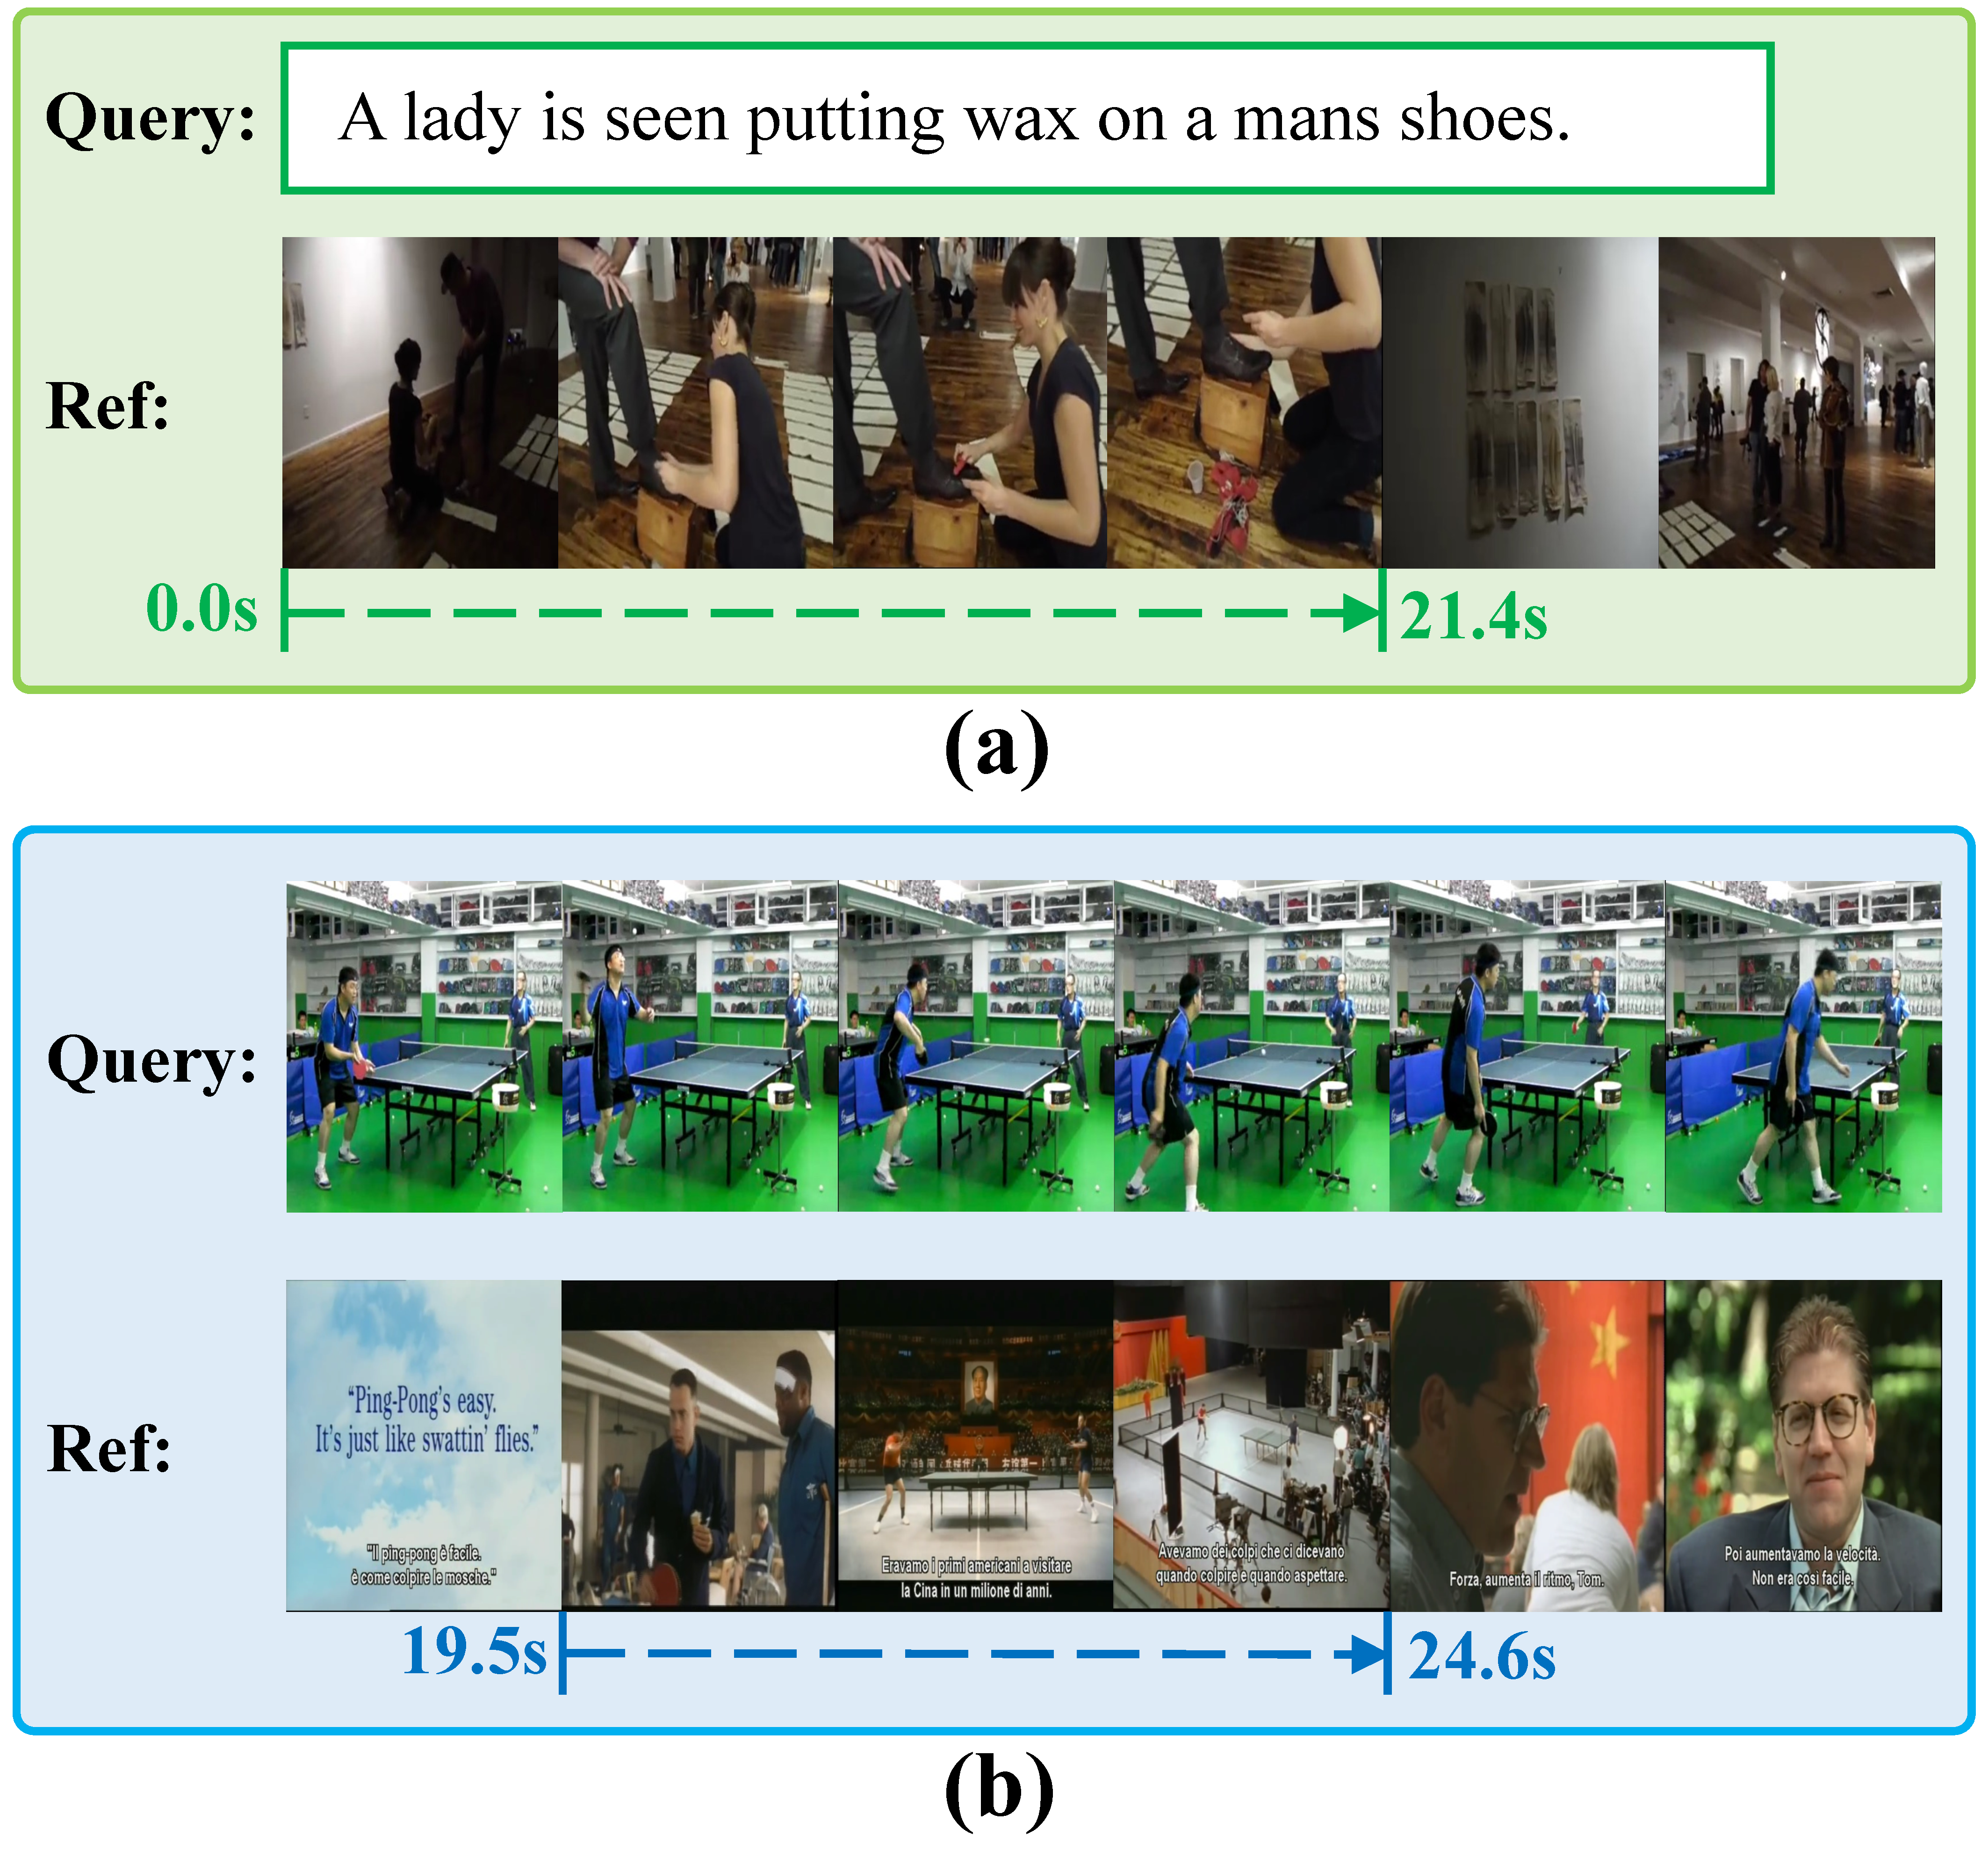
\includegraphics[width=0.8\linewidth]{chapter6/res/qbvl.pdf}
    \caption{两种不同的视频片段检索任务}
    \label{ch6:fig:qbvl}
\end{figure}

到目前为止,绝大多数的视频片段检索方法都属于\textbf{自顶向下}的方法:它们将视频序列切分为众多的候选视频片段,然后对每个候选片段进行分类和回归。具体来说,这些自顶向下的方法又可以细分为两类:(1)滑窗型(sliding-window-based)~\cite{gao2017tall,anne2017localizing,liu2018attentive,liu2018cross,ge2019mac,chen2019semantic,xu2019multilevel,zhang2019exploiting}:它们预先定义一系列不同大小的滑窗,然后利用滑窗密集地将视频“显式”地切分成若干候选视频片段,最后分别对查询和候选片段提取特征。这样,视频片段检索任务就转变为一个相似度匹配问题。但是这类方法忽略了视频中每个视频帧与其他周围帧之间的内在联系,并且通常这些周围帧对视频语义理解有着巨大的帮助~\cite{wu2019long}。(2)锚框型(anchor-based)~\cite{chen2018temporally,zhang2019man}:它们不像滑窗型直接对视频进行预先切分,而是在每个视频帧上定义若干个锚框,然后对每个锚框内的视频进行分类和回归。为了充分地利用周围的视频帧,它们通常采用递归神经网络将所有的视频帧进行串接。这类方法可以看成是基于锚框型的目标检测方法~\cite{ren2015faster}在视频领域的拓展。

尽管这些自顶向下的模型(包括滑窗型和锚框型)可以在多个视频片段检索数据集上达到当时最好的性能,但是这类方法本质上仍然有许多一些不可避免的缺点:(1)最终的视频片段检索结果受预先定义的规则影响较大(如滑窗或锚框的大小、数量等);(2)为了尽可能的提高召回率,模型必须增大滑窗或锚框数量,这将导致整个计算量增大、定位速度慢。


\begin{figure}[t]
    \centering
    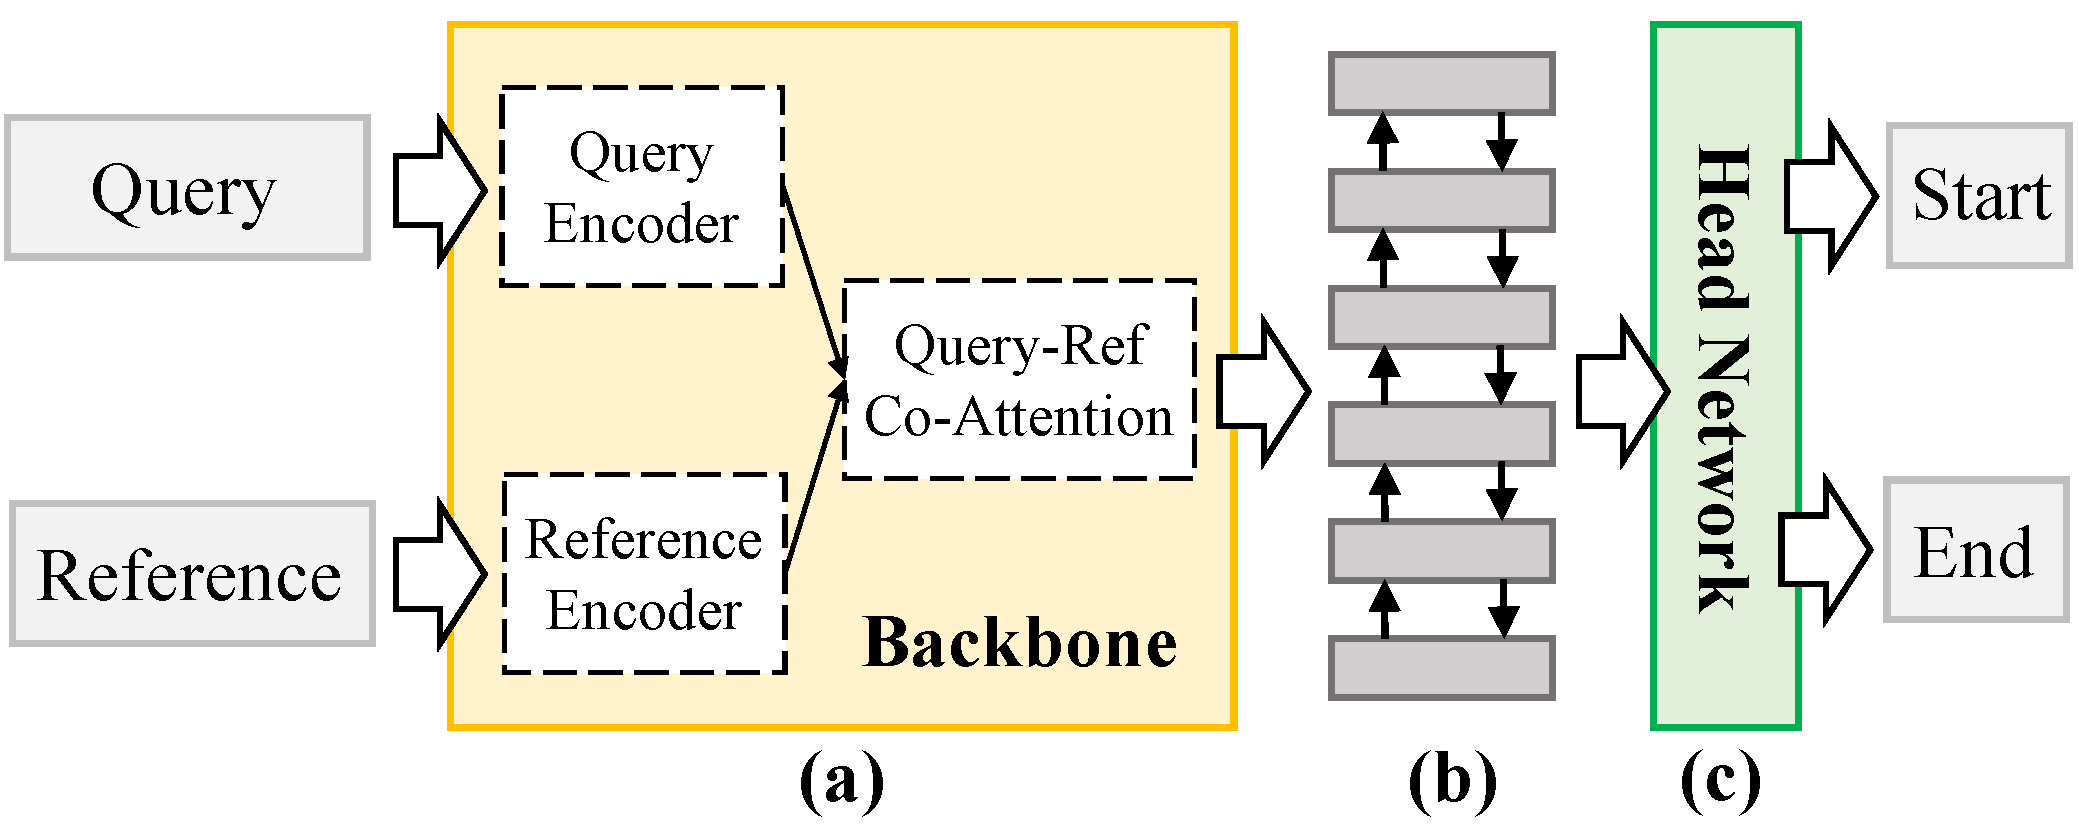
\includegraphics[width=0.8\linewidth]{chapter6/res/sparse_bu.pdf}
    \caption{典型的稀疏型自底向上视频片段检索模型}
    \label{ch6:fig:sparse_bu}
\end{figure}


为了消除上述这些缺点,一些视频片段检索方法~\cite{chen2019localizing,yuan2019find,feng2018video}开始借鉴自然语言处理领域中阅读理解任务(reading comprehension)的方法\cite{xiong2017dynamic,xiong2018dcn+,yu2018qanet},用一种\textbf{稀疏型自底向上}的网络直接预测两个边界的概率。如图~\ref{ch6:fig:sparse_bu}所示,一个典型的稀疏型自底向上模型通常包含两个组成部分:骨干网络(图~\ref{ch6:fig:sparse_bu}(a))和头网络(图~\ref{ch6:fig:sparse_bu}(c))。骨干网络通常会使用协同注意力机制(co-attention mechanism)来融合查询特征和每个视频帧的特征,它的输出是融合后的特征帧序列(图~\ref{ch6:fig:sparse_bu}(b))。为了后续的头网络能够直接对视频帧序列中每一帧预测边界概率,融合后的特征帧序列往往需要保持和输入视频帧相同的长度。尽管这种稀疏型自底向上的方法可以避免自顶向下方法的缺点,但是它们的性能目前却仍然低于自顶向下方法。尤其是对于长视频(如:数据集TACoS),这种差距往往更加明显。在本章,我们认为自底向上方法的性能低于自顶向下方法的主要原因来自于目前骨干网络和头网络的不合理设计:

(i)骨干网络(Backbone Network):对于骨干网络的设计,目前的稀疏型自底向上模型主要有两个缺点:(1)每个视频通常包含丰富的场景变化,即不同的视频场景分布在视频的不同位置中。因此,理解视频中不同场景的变化以及场景之间的关系对于充分理解视频内容十分重要。然而,目前的方法通常使用递归神经网络来编码视频帧特征,忽略了场景之间的内在联系。(2)为了方便头网络对每一帧进行预测,骨干网络需要让融合后的特征帧序列保持和原始视频帧相同的长度,这容易导致每个视频帧特征只编码局部的语义信息,而忽略全局的视频语义信息~\cite{chen2018encoder,lin2017feature}。

(ii)头网络(Head Network):对于头网络的设计,目前的稀疏型自底向上模型主要有三个缺点:(1)两个边界时刻(起始时刻和终止时刻)的预测是相互独立的,即模型预测边界时忽略了两个边界之间视频内容的连贯性。如图~\ref{ch6:fig:headnetwork_motivation}(a),时刻B和时刻D的视频帧有非常相似的场景内容。因此,模型很容易将最终结果预测为(A$\to$D),即使在时刻(B$\to$C)之间存在明显的视频场景内容变化。(2)在训练过程中,正样本和负样本的数量极度不均。因为视频的长度通常较长(如:数据集TACoS中每个视频的平均长度为9000帧),而其中只有两个边界帧为正样本(如图~\ref{ch6:fig:headnetwork_motivation}(b))。(3)即使没有查询输入的约束,对视频中的动作边界进行定位本身仍然是目前尚未解决的开放性难题~\cite{shou2018online}。因为它不仅需要判断每个视频帧内容和查询内容是否相关,同时需要判断该视频帧是否为动作边界。

\begin{figure}[t]
    \centering
    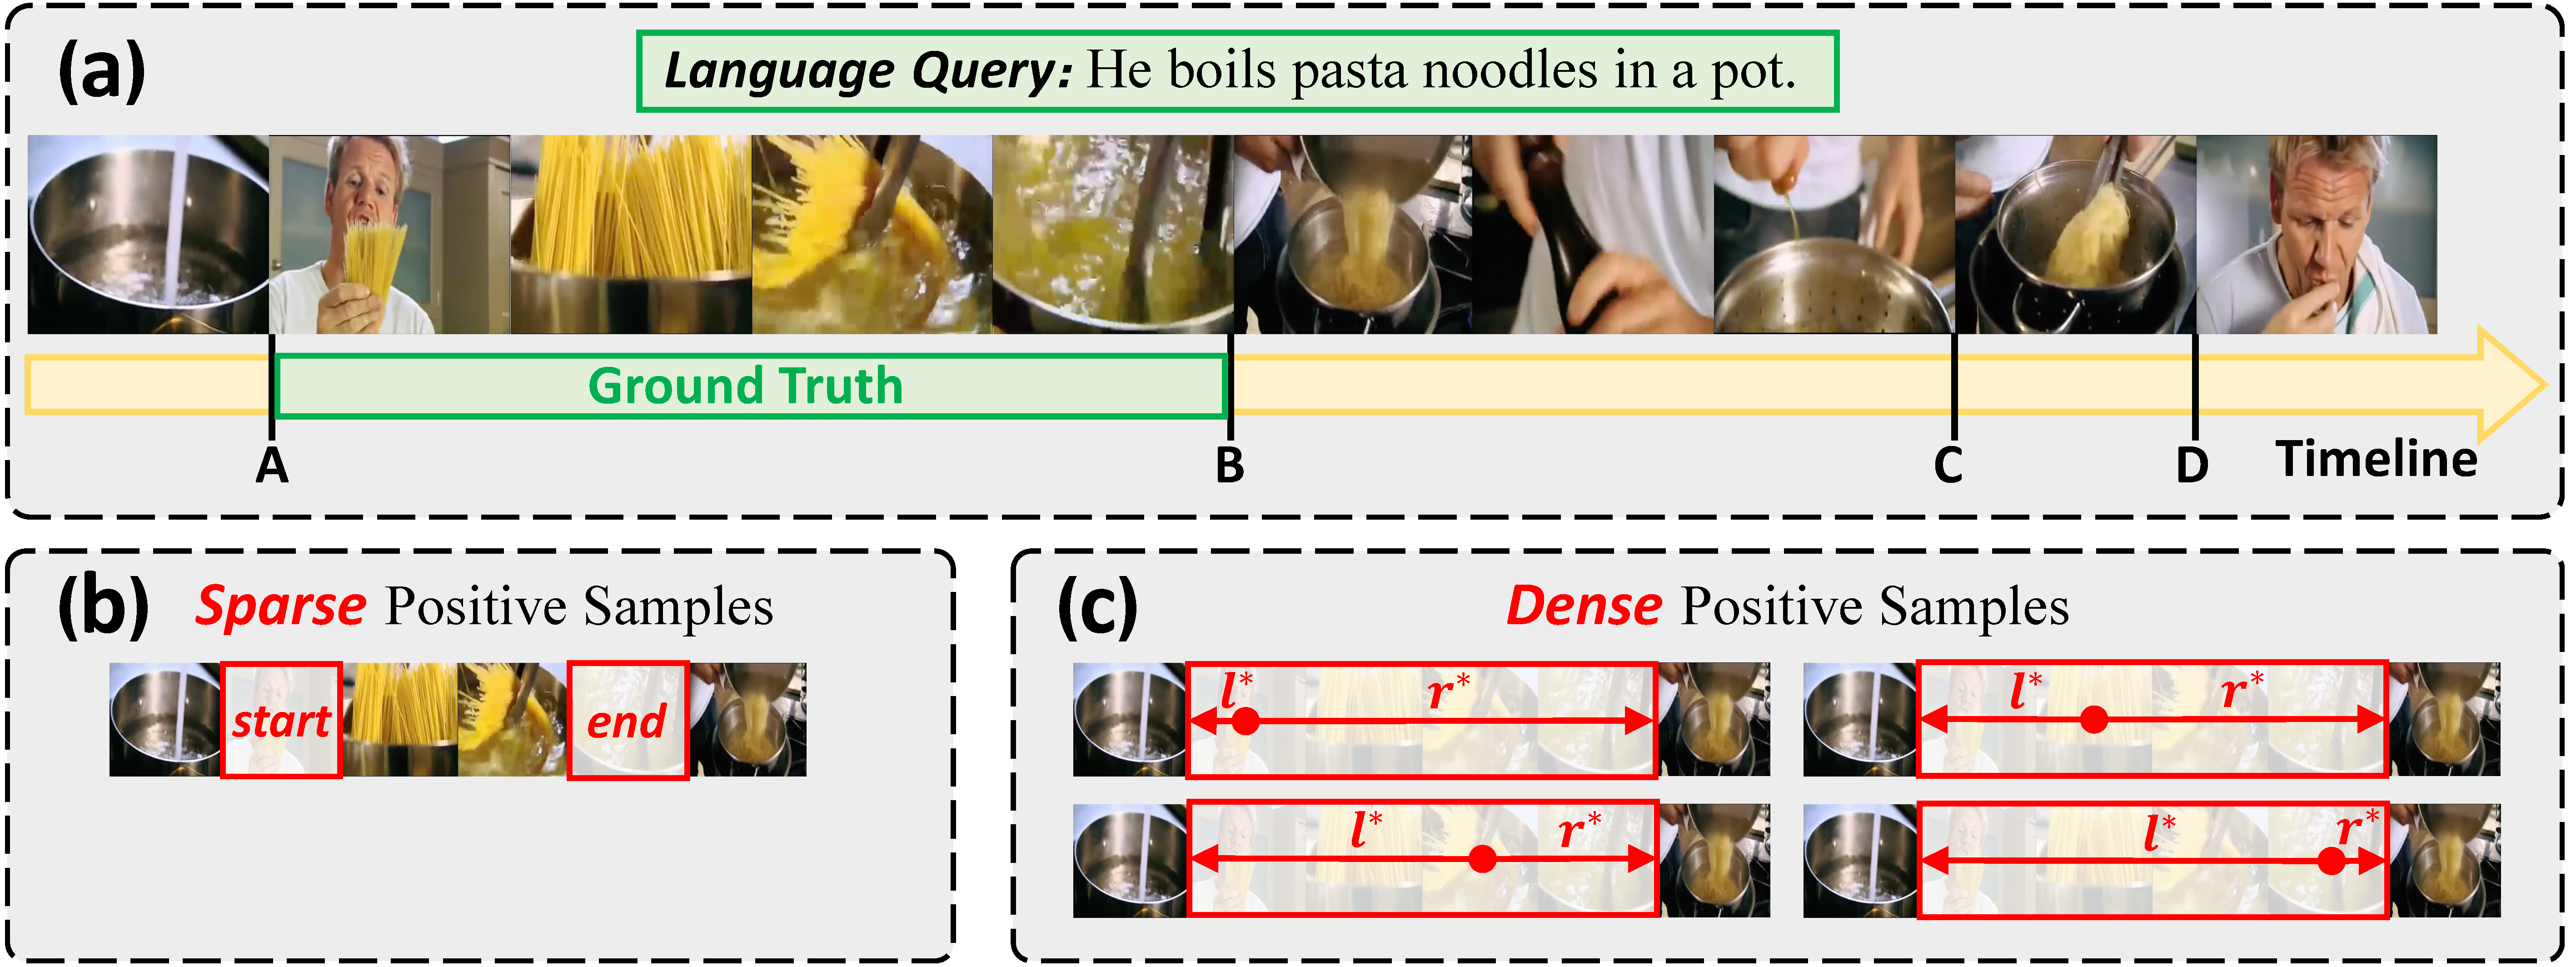
\includegraphics[width=0.98\linewidth]{chapter6/res/headnetwork_motivation.pdf}
    \caption{一个基于语句查询的视频片段检索示例}
    \label{ch6:fig:headnetwork_motivation}
\end{figure}


在本章,我们针对目前稀疏型自底向上模型的缺点,提出了一种全新的密集型自底向上网络:基于图特征金字塔的密集型预测(Graph-FPN with Dense Prediction, GDP)。对于骨干网络,模型GDP引入一个图特征金字塔层来增强骨干网络输出的特征帧序列(图~\ref{ch6:fig:sparse_bu}(b))。模型GDP首先构建一个金字塔多尺度特征,然后将不同尺度的特征序列映射到一个高语义的场景空间中,并利用图卷积对场景空间中的节点进行特征融合。图卷积不仅可以充分地利用不同语义场景之间的内在联系,同时可以消除不同尺度下特征的语义差。最后,这些场景空间的特征重新映射得到新的特征序列。对于头网络,我们将起始时刻到终止时刻中间的每一帧都看成是正样本帧。对于每个正样本帧,模型GDP包含一个回归网络来预测从当前帧到两个边界帧各自的距离。这样的设计一方面可以缓解训练过程中正负样本极度不均的问题,另一方面由于两个边界预测来自于同一个特征,也可以避免陷入独立预测的局部最优。同时,模型GDP包含一个置信网络分支来预测当前帧与查询的关联度,可以将边界帧预测任务分离成内容关联度判断和边界回归两个子任务,降低视频片段检索任务的难度。

我们在四个常用的视频片段检索数据集(TACoS~\cite{regneri2013grounding}、Charades-STA~\cite{gao2017tall}、ActivityNet Captions~\cite{krishna2017dense}和Activity-VRL~\cite{feng2018video})中验证了模型GDP的有效性。在多个不同的评估指标下,模型GDP都达到了目前最佳的实验性能。

\section{基于图特征金字塔的密集型预测}

给定一个视频序列$\mathcal{V}$和查询输入$\mathcal{Q}$,视频片段检索任务需要预测出两个边界时刻($t_s, t_e$),满足从$t_s$到$t_e$之间的视频片段内容与查询内容一致。在本节,我们将首先介绍模型GDP中的各个组合部分~\ref{ch6:fig:dense_bu},包括骨干网络(a)、图特征金字塔层(b)和密集型头网络(c)。之后,我们再介绍模型GDP的训练和测试过程。

\begin{figure}[t]
    \centering
    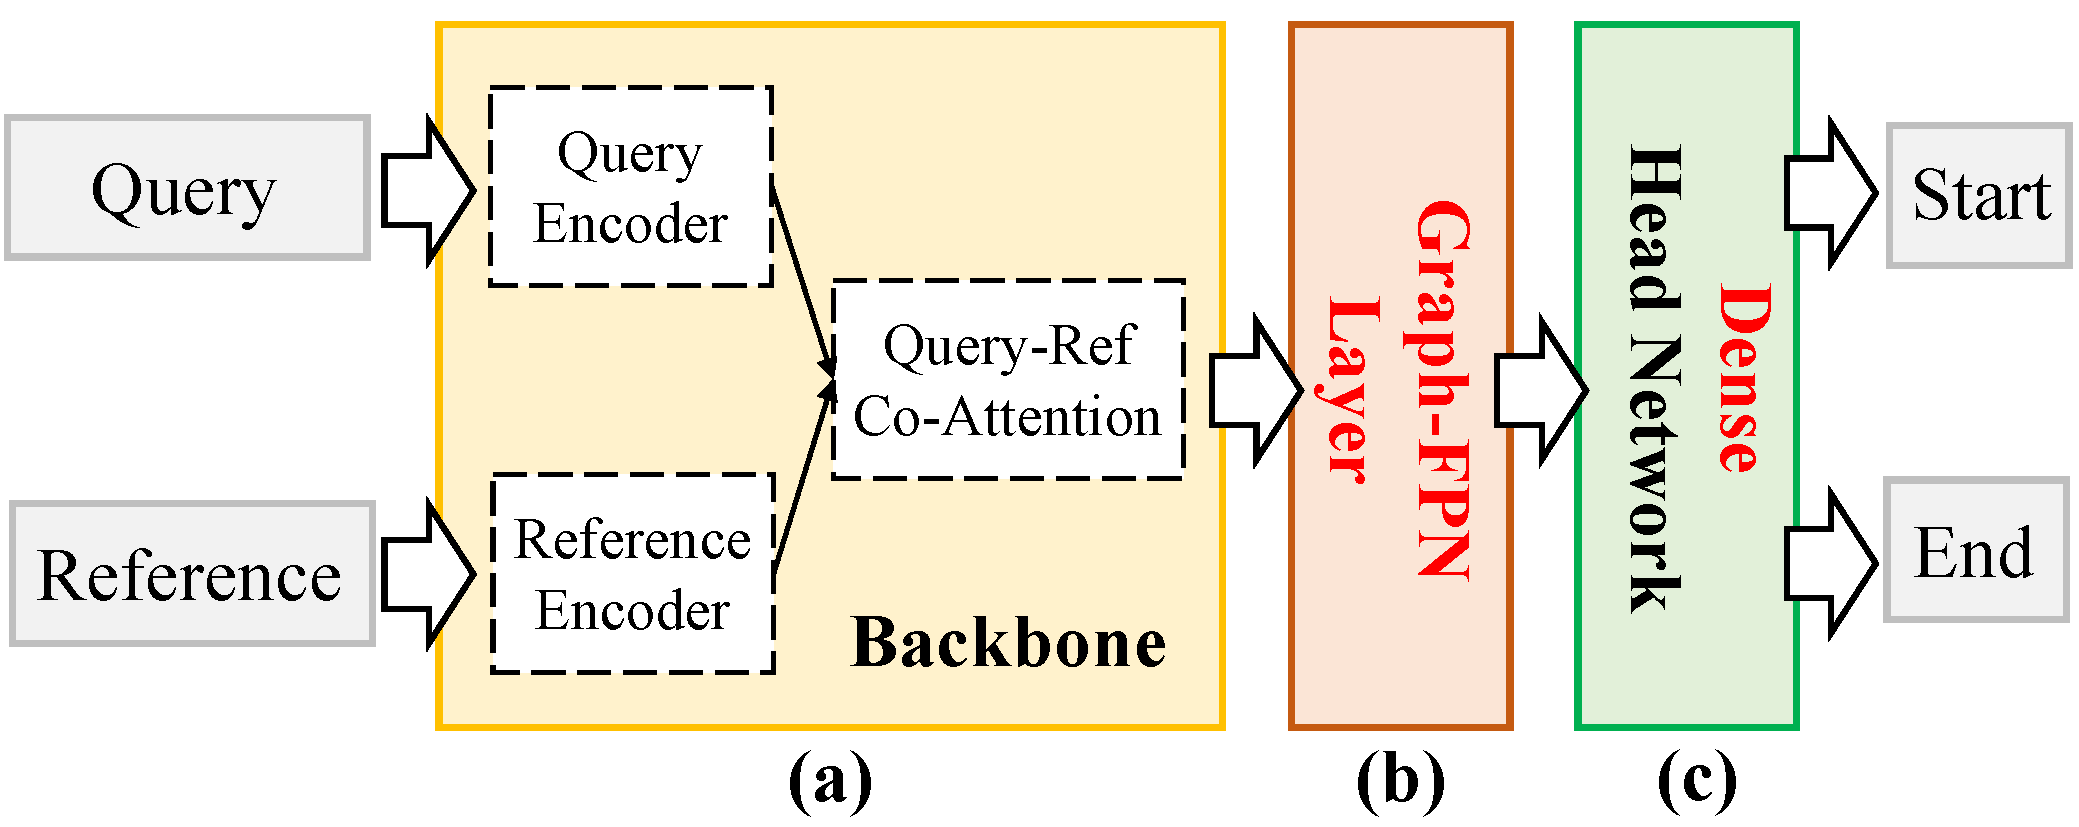
\includegraphics[width=0.8\linewidth]{chapter6/res/dense_bu.pdf}
    \caption{典型的稀疏型自底向上视频片段检索模型}
    \label{ch6:fig:dense_bu}
\end{figure}

\subsection{骨干网络}
模型GDP的骨干网络使用模型QANet~\cite{yu2018qanet}来融合查询和视频的特征。如图~\ref{ch6:fig:qanet}所示,模型QANet共有两个输入:查询输入特征$\bm{Q} = \{\bm{q}_n\}^N_{n=1}$和视频序列特征$\bm{V}=\{\bm{v}_i\}^T_{i=1}$,其中$N$和$T$分别表示查询和视频的长度。具体来说,模型QANet包含四个主要部分:

(1)查询特征编码器:查询特征编码器包含多个特征编码层对输入的查询特征$\bm{Q}$进行编码。如图~\ref{ch6:fig:qanet}(b)所示,每个特征编码层由多个卷积层、层归一化层、自注意力层和全连接层组成。查询特征编码器的输出是$\bm{\tilde{Q}}=\{\bm{\tilde{q}}_n\}^N_{n=1}$。

(2)视频特征编码器:视频特征编码器对输入的视频特征$\bm{V}$进行编码。其结构和查询特征编码器完全相同,即由多个特征编码层组成(如图~\ref{ch6:fig:qanet}(b))。视频特征编码器的输出是$\bm{\tilde{V}} = \{\bm{\tilde{v}}_i\}^T_{i=1}$。

(3)查询-视频协同注意力层:查询-视频协同注意力层包含一个协同注意力机制来融合查询特征$\bm{\tilde{Q}}=\{\bm{\tilde{q}}_n\}^N_{n=1}$和视频特征$\bm{\tilde{V}} = \{\bm{\tilde{v}}_i\}^T_{i=1}$。具体来说,它先计算一个相似矩阵$\bm{S}\in\mathbb{R}^{T\times N}$,其中每个元素$\bm{S}_{ij}$表示$\bm{\tilde{v}}_i$和$\bm{\tilde{q}}_j$之间的相似度。然后可以得到两个加权特征:
\begin{equation}
  \bm{A} = \bar{\bm{S}} \cdot \tilde{\bm{Q}}, \quad \bm{B} = \bar{\bm{S}} \cdot \bar{\bar{\bm{S}}}^T \cdot \tilde{\bm{V}},
\end{equation}
其中$\bar{\bm{S}}$和$\bar{\bar{\bm{S}}}$分别是对$\bm{S}$按行和按列进行归一化。

\begin{figure}[t]
    \centering
    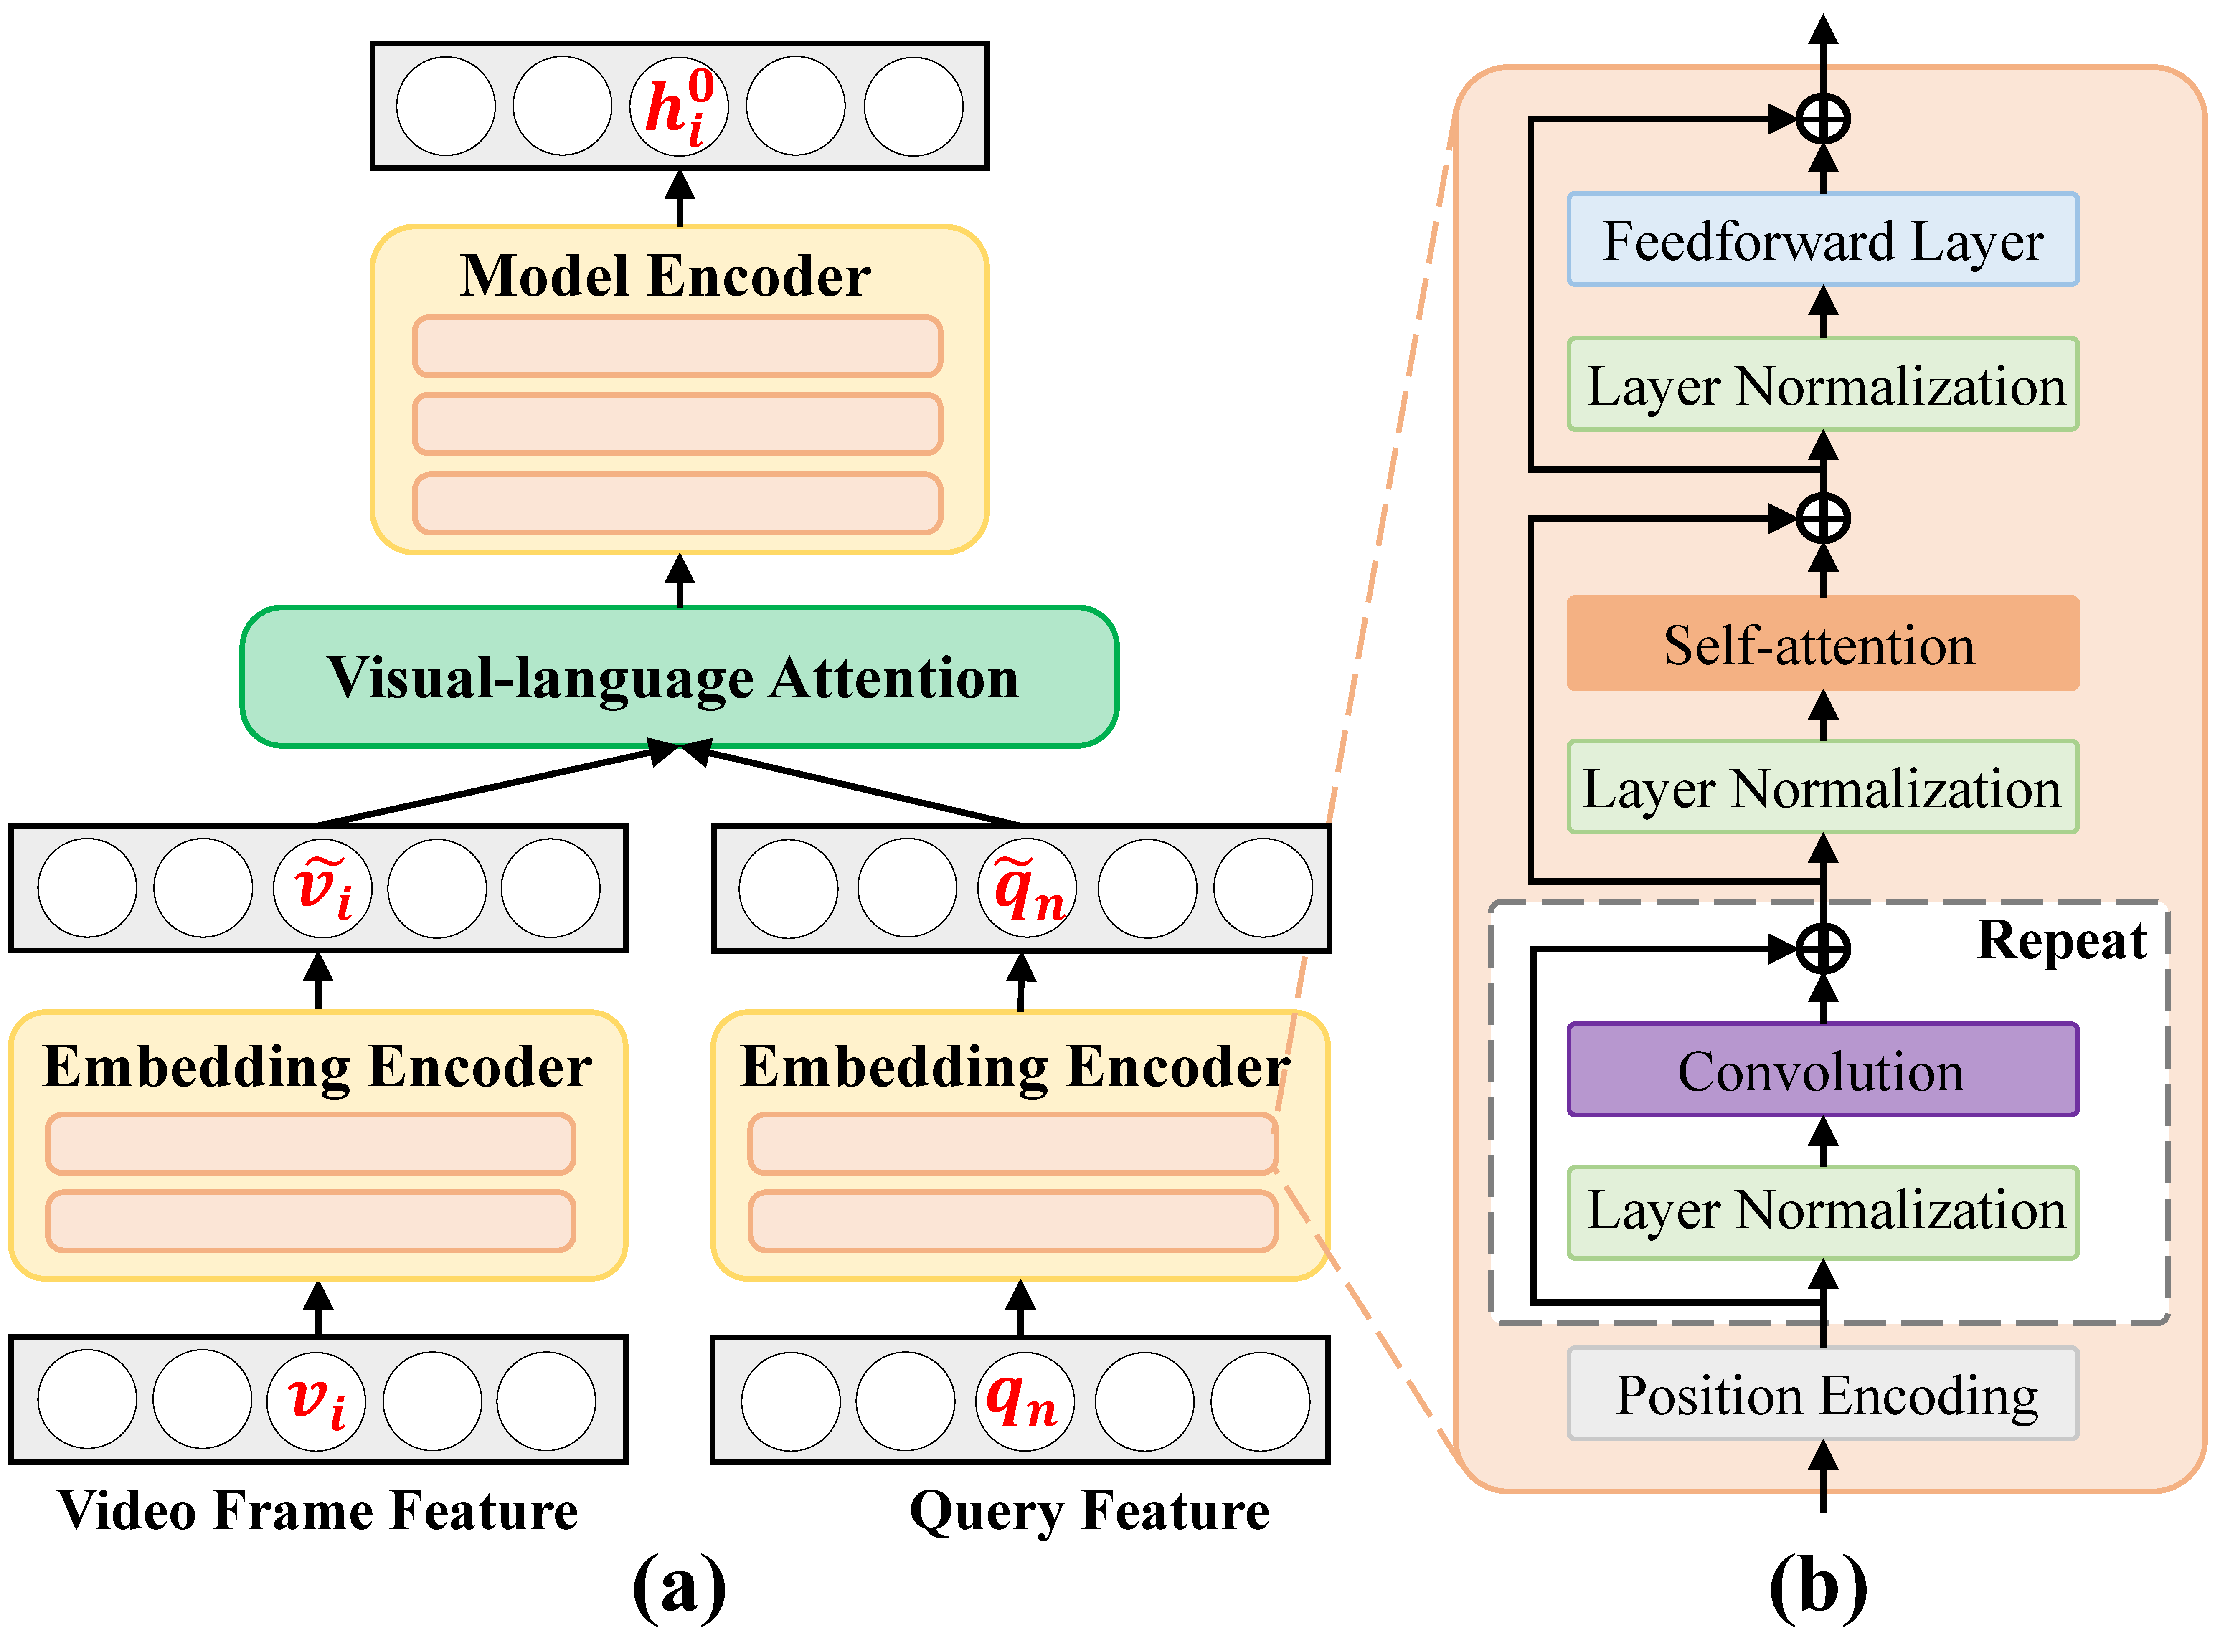
\includegraphics[width=0.8\linewidth]{chapter6/res/qanet.pdf}
    \caption{模型QANet的结构细节}
    \label{ch6:fig:qanet}
\end{figure}

(4)融合特征编码器:给定两个注意力权重矩阵$\bm{A}$和$\bm{B}$,融合特征编码器开始对融合后的特征进行编码。融合特征编码器同样由多层特征编码层(图~\ref{ch6:fig:qanet}(b))组成。融合特征编码器的输入是一个特征序列,它的第$i$个特征为$[\bm{v}_i, \bm{a}_i, \bm{v}_i\odot \bm{a}_i, \bm{v}_i\odot \bm{b}_i]$,其中$\bm{a}_i$和$\bm{b}_i$分别是矩阵$\bm{A}$和$\bm{B}$的第$i$行,$\odot$是元素积,$[,]$是向量连接符。融合特征编码器的输出为$\bm{H}_0=\{\bm{h}^0_i\}^T_{i=1}$,$\bm{H}_0 \in \mathbb{R}^{T\times D}$,其中每个特征$\bm{h}^0_i \in \mathbb{R}^D$都编码了查询信息。现有的稀疏型自底向上模型通常直接将$\bm{H}_0$作为头网络的输入,相反,模型GDP包含一个图特征金字塔层对特征$\bm{H}_0$进行增强。值得注意的是,模型GDP兼容任意的骨干网络。

\begin{figure}[t]
    \centering
    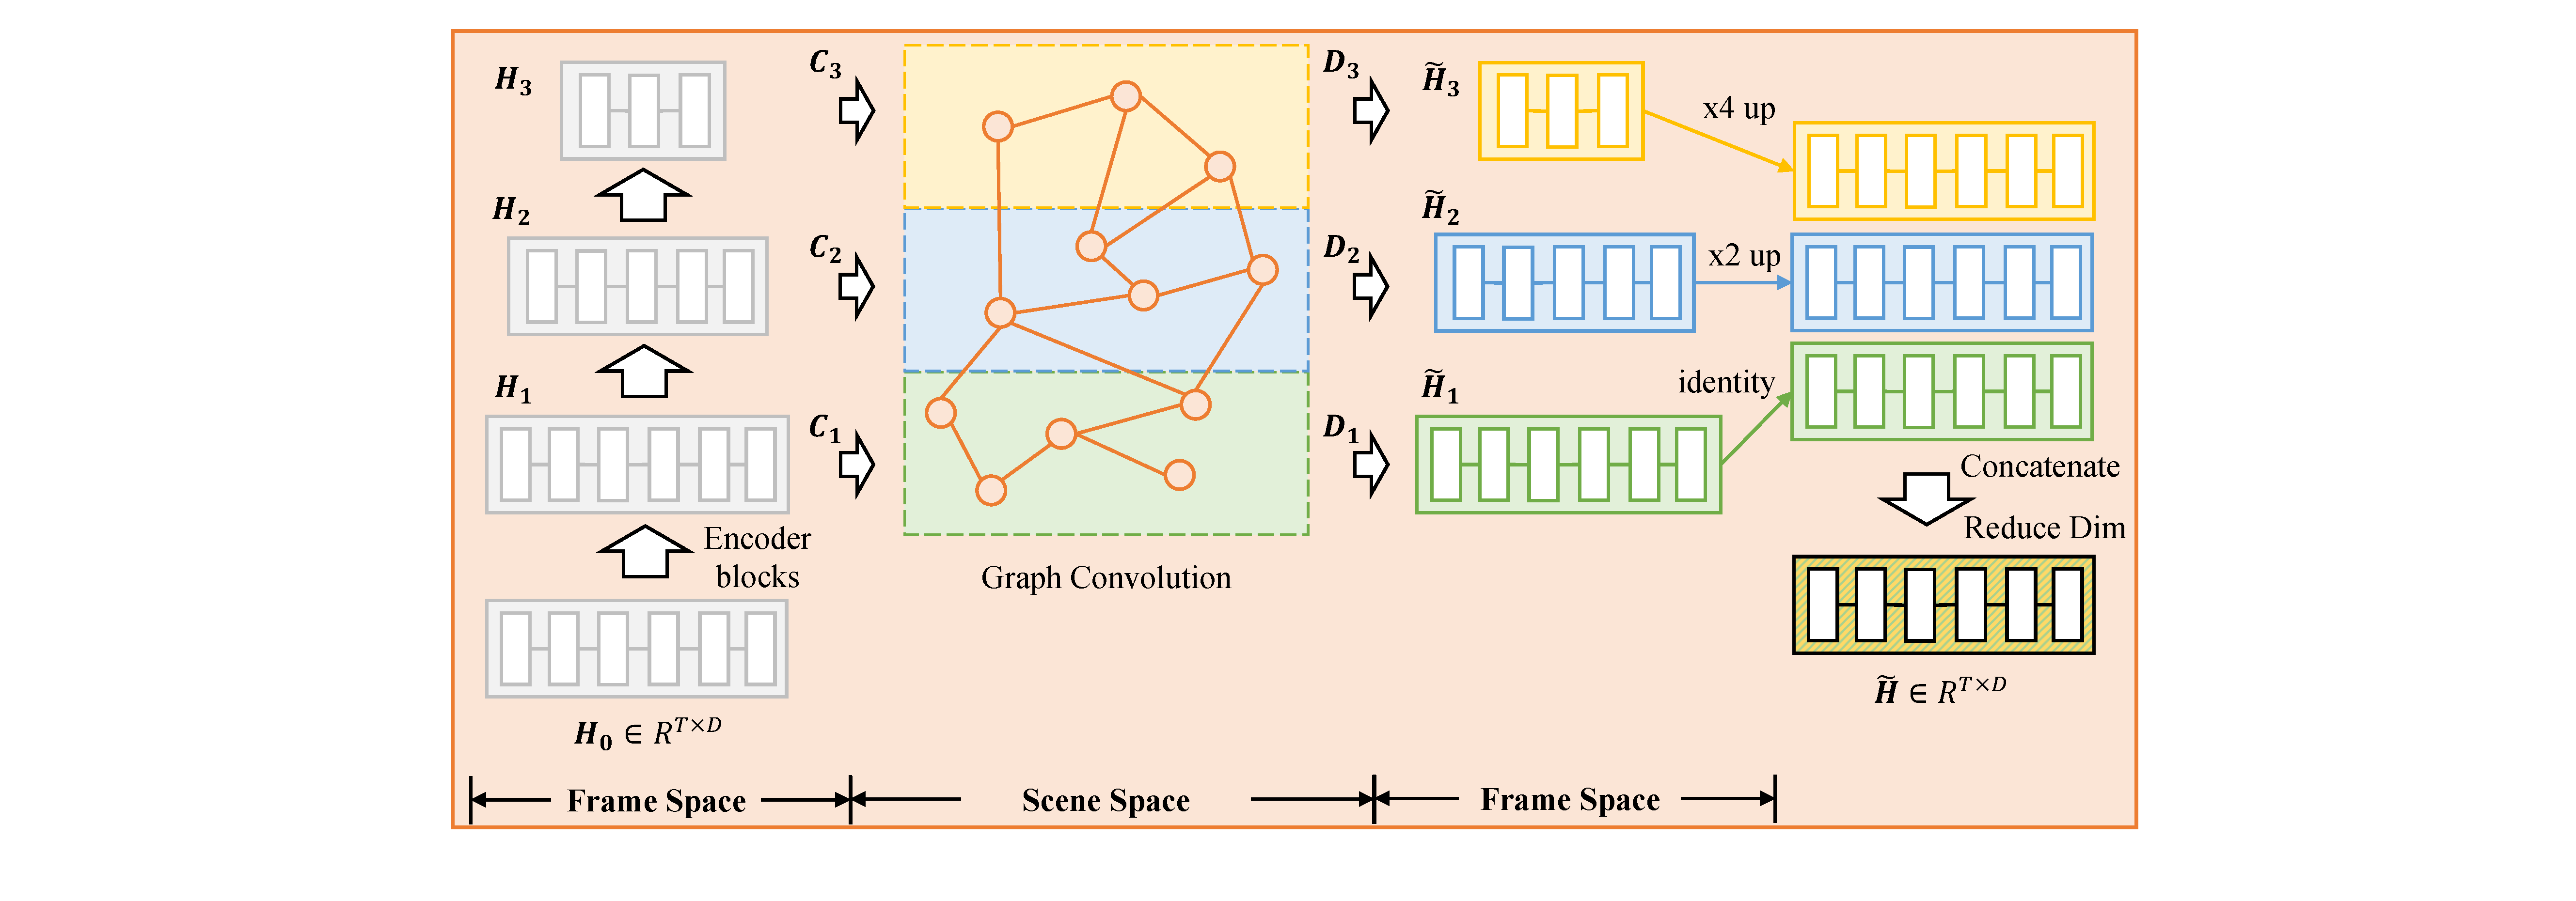
\includegraphics[width=0.98\linewidth]{chapter6/res/graph_fpn.pdf}
    \caption{模型GDP中的图特征金字塔层}
    \label{ch6:fig:graph_fpn}
\end{figure}

\subsection{图特征金字塔层}
如图~\ref{ch6:fig:graph_fpn}所示,图特征金字塔层主要包含四个步骤来增强骨干网络输出$\bm{H}_0$:

(1)特征金字塔的构建:给定特征帧序列$\bm{H}_0$,我们首先通过逐渐减少特征序列长度来构建特征金字塔$\{\bm{H}_1 \in \mathbb{R}^{T_1\times D}, \bm{H}_2 \in \mathbb{R}^{T_2\times D}, \bm{H}_3 \in \mathbb{R}^{T_3\times D}\}$,其中$T_{i+1} = T_i/2$。我们同样使用相同的多个特征编码层(如图~\ref{ch6:fig:qanet}(b))和一个额外的步长为2的卷积层将特征$\bm{H}_i$转换为$\bm{H}_{i+1}$。

(2)帧空间到场景空间:在得到多个尺度的特征$\{\bm{H}_1, \bm{H}_2, \bm{H}_3\}$之后,我们将这些特征从原始的帧空间映射到场景空间。以$\bm{H}_2 = \{\bm{h}^2_i\}^{T_2}_{i=1}$为例,我们希望得到一系列场景空间特征$\bm{X}_2 = f_2(\bm{H}_2) \in \mathbb{R}^{N_2\times D}$,其中$N_2$表示场景空间在该尺度特征的节点数量,映射函数$f_2(\cdot)$是对原始输入特征的线性组合:
\begin{equation} \label{ch6:eq:eq_2}
    \bm{x}^2_i = \bm{c}^2_i \bm{H}_2 = \sum\nolimits_j c^2_{ij}\bm{h}^2_j,
\end{equation}
其中$\bm{C}_2 = [\bm{c}^2_1, ..., \bm{c}^2_{N_2}]$,$\bm{C}_2 \in \mathbb{R}^{N_2\times T_2}$。$\bm{C}_2$由$\bm{H}_2$经过一个$1\times1$卷积层得到。类似地,我们可以通过$\bm{H}_1$、$\bm{H}_3$分别得到$\bm{X}_1 \in \mathbb{R}^{N_1\times D}$和$\bm{X}_3 \in \mathbb{R}^{N_3\times D}$。

(3)场景空间图卷积:当把不同尺度的特征都从帧空间映射到场景空间之后,我们使用图卷积(graph convolution)~\cite{kipf2017semi}里编码不同场景间的关系。具体来说,我们将所有的$N_{total}$节点($N_{total} = N_1 + N_2 + N_3$)看成一个全连接图,然后利用图卷积进行参数更新:
\begin{equation}
    \bm{Y} = ((\bm{I}-\bm{A}_{adj})\bm{X})\bm{W},
\end{equation}
其中,$\bm{X} = [\bm{X}_1; \bm{X}_2; \bm{X}_3] \in \mathbb{R}^{N_{total}\times D}$是场景空间所有节点特征的集合,[;]表示矩阵按行连接符,$\bm{W}\in \mathbb{R}^{D\times D}$是可学习的映射矩阵,$\bm{A}_{adj} \in \mathbb{R}^{N_{total}\times N_{total}}$是可学习的邻接矩阵,$\bm{I}$是大小与$\bm{A}_{adj}$相同的单位矩阵。

(4)场景空间到帧空间:给定场景空间特征$\bm{Y} = [\bm{Y}_1; \bm{Y}_2; \bm{Y}_3]$,我们重新将特征从场景空间映射回帧空间。以$\bm{Y}_2$为例:
\begin{equation}
    \tilde{\bm{h}}^2_i = \bm{d}^2_i \bm{Y}_2 = \sum\nolimits_j d^2_{ij} y^2_j,
\end{equation}
其中$\bm{D}_2 = [\bm{d}^2_1, ..., \bm{d}^2_{T_2}]$,$\bm{D}_2 \in \mathbb{R}^{T_2 \times N_2}$。为了减少模型的参数量,我们设定$\bm{C}_i=\bm{D}^T_i$。因此,我们可以得到增强的特征序列$\{\tilde{\bm{H}}_1, \tilde{\bm{H}}_2, \tilde{\bm{H}}_3\}$。最后,通过增大$\tilde{\bm{H}}_1$和$\tilde{\bm{H}}_2$的长度,并将所有的特征连接起来,得到输出特征$\tilde{\bm{H}} \in \mathbb{R}^{T_1 \times D}$。


\subsection{密集型头网络}

\begin{wrapfigure}{r}{0.3\linewidth}
    \centering
        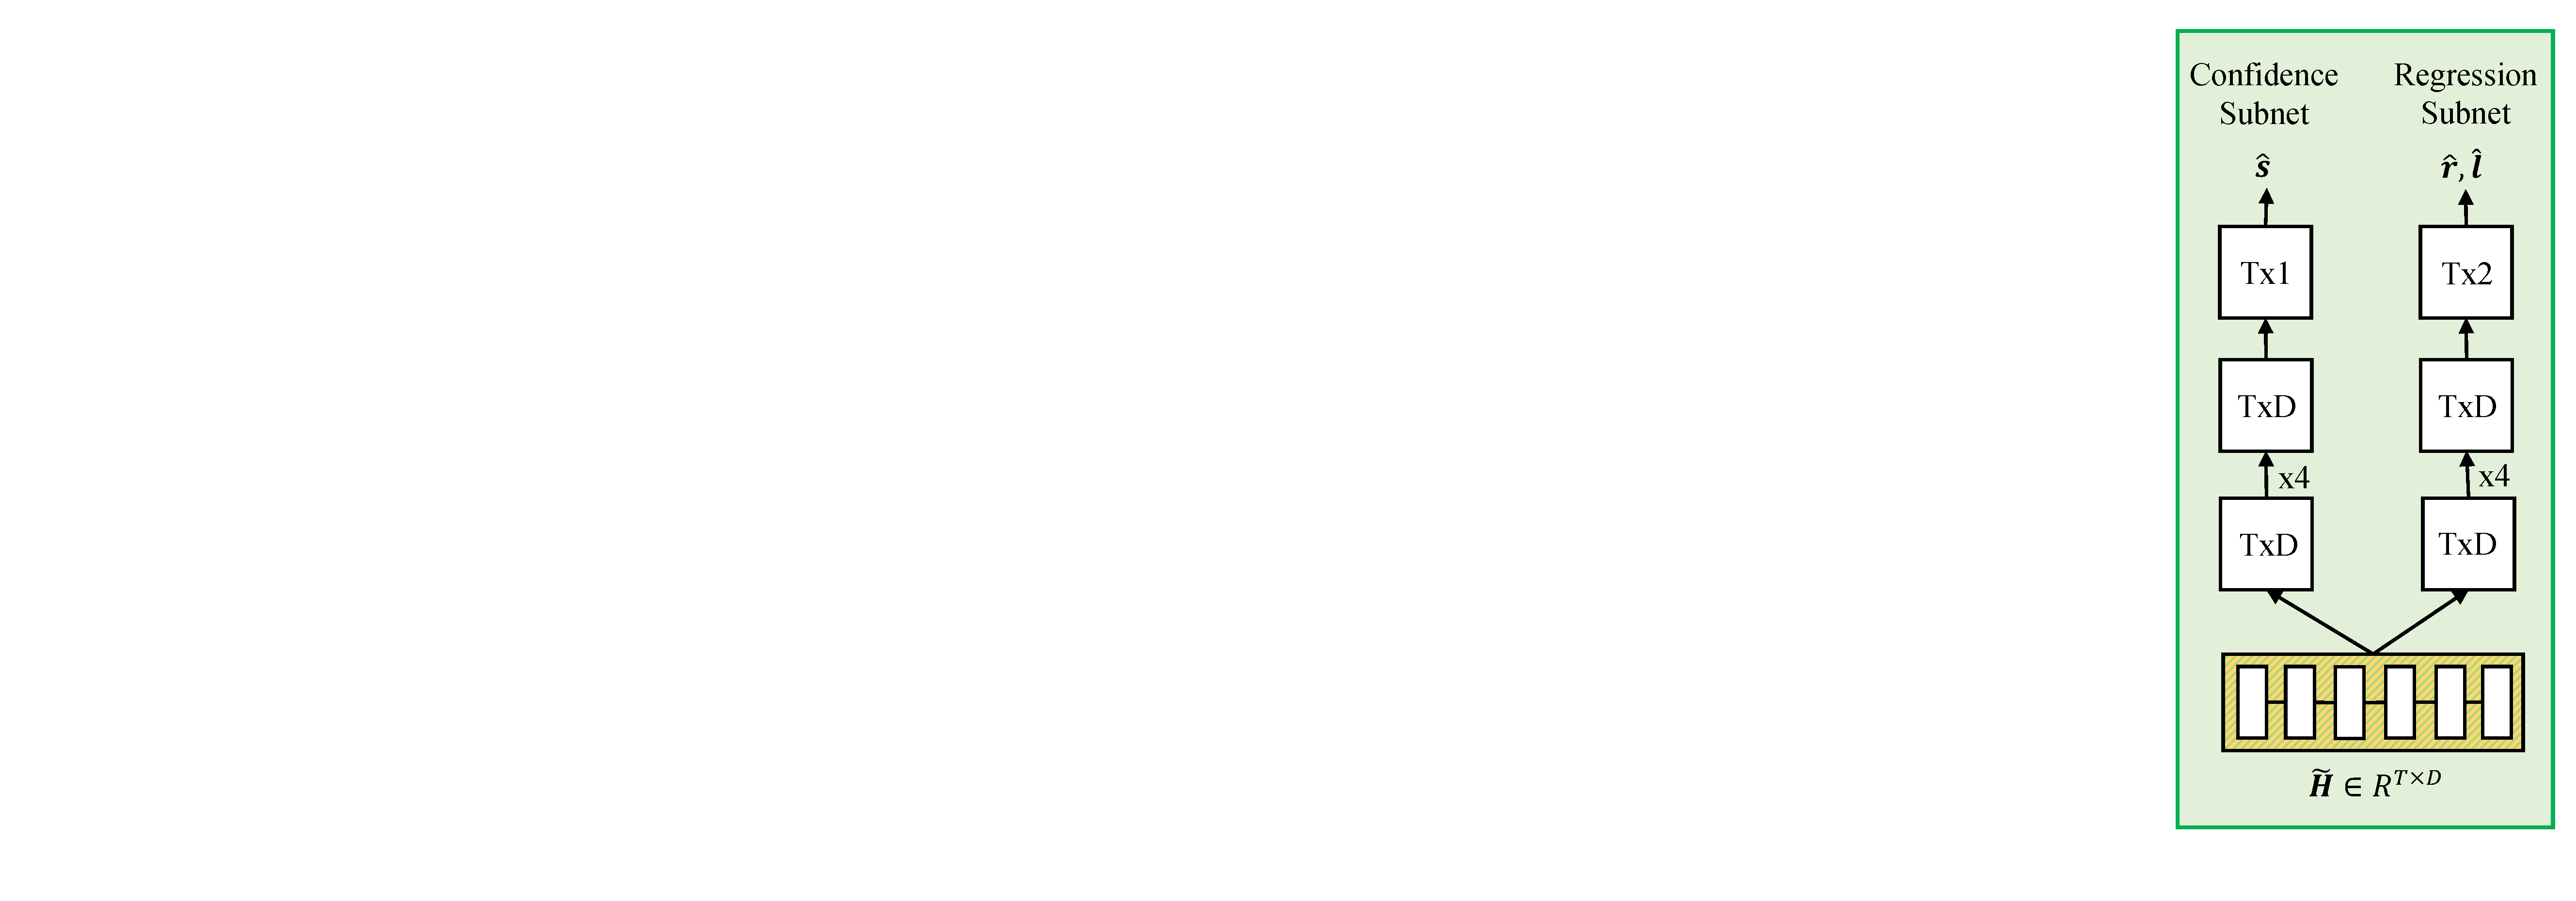
\includegraphics[width=0.9\linewidth]{chapter6/res/head_network.pdf}
    \captionof{figure}{模型GDP中的密集型头网络}
    \label{ch3:fig:head_network}
\end{wrapfigure}

与稀疏型自底向上模型不同,模型GDP将起始时刻和终止时刻之间的每一帧都看成是正样本。对于每一帧,模型GDP分别使用两个分支网络(如图~\ref{ch3:fig:head_network}):

(1)回归分支网络(Regression Subnet):对于每一帧,回归分支网络分别预测当前帧位置到两个边界帧的距离。给定图特征金字塔层的输出$\tilde{\bm{H}}$,回归分支网络使用四个通道数为$D$的$1\times3$的卷积层和一个通道数为1的$1\times3$卷积层。最后用非线性激活函数sigmoid输出预测的两侧边界距离。对于回归分支网络,我们只使用正样本计算预测损失。对于第$i$帧,假设人工标注的结果为($t_s, t_e$)(即:$t_s \leq i \leq t_e$),回归分支网络的预测目标设为:
\begin{equation}
    l^*_i = i - t_s, \quad r^*_i = t_e - i,
\end{equation}
其中$l^*_i$和$r^*_i$分别表示从第$i$帧到左右两侧边界的距离。

(2)置信分支网络(Confindence Subnet):虽然每一帧都有独立的边界预测,但是不同帧的预测置信度往往不同。例如,离起始时刻比较近的帧预测起始时刻的置信度通常比预测终止时刻的置信度要高。基于这一观察,我们认为中心帧对两个边界预测的综合置信度最高。因此,我们将置信分支的目标设为:
\begin{equation}
s^*_i=\left\{
    \begin{aligned}
        & \frac{\min(l^*_i, r^*_i)}{\max(l^*_i, r^*_i)}, & t_s \leq i \leq t_e \\
        & 0.  & i < t_s ~\text{or}~ i > t_e \\
    \end{aligned}
    \right.
\end{equation}

\begin{figure}[t]
    \centering
    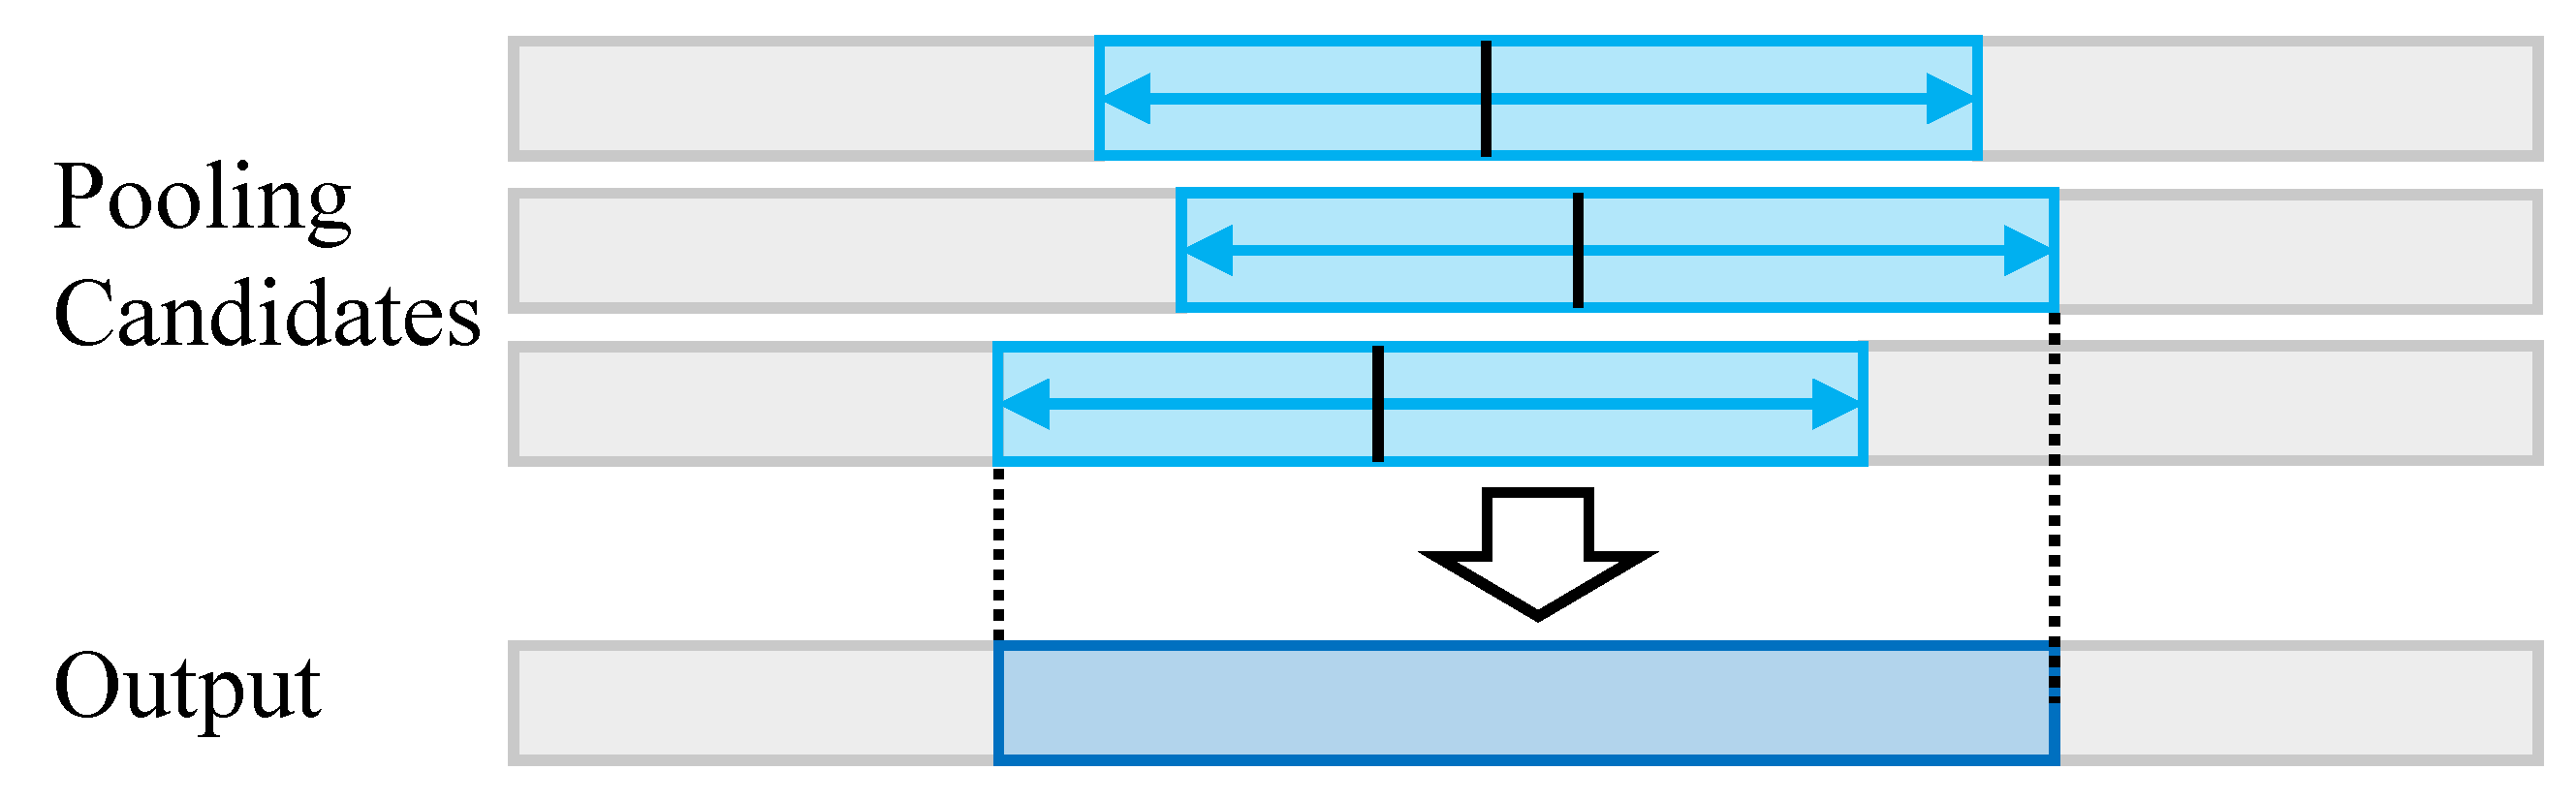
\includegraphics[width=0.8\linewidth]{chapter6/res/temporal_pooling.pdf}
    \caption{时域池化示意图}
    \label{ch6:fig:temporal_pooling}
\end{figure}

\subsection{训练阶段和测试阶段}

\textbf{\kaishu{损失函数}}:给定所有特征序列帧的两个分支网络预测结果$\{(\hat{t}_i, \hat{s}_i)\}^T_{i=1}$和相应人工标注的目标$\{(t^*_i, s^*_i)\}^T_{i=1}$,整个模型GDP的训练损失函数为:
\begin{equation}
    L = \frac{1}{T}L_{conf}(\hat{s}_i, s^*_i) + \frac{1}{T_p}\mathbf{1}_{\{s^*_i>0\}}L_{reg}(\hat{t}_i, t^*_i),
\end{equation}
其中,$T$和$T_p$分别表示总样本帧和正样本帧的数量,$\mathbf{1}_{\{s^*_i>0\}}$为指示函数,当$s^*_i>0$时值为1,否则值为0。置信分支网络的分类损失函数$L_{conf}$为是二值化交叉熵函数,回归分支网络的回归损失函数$L_{reg}(\hat{t}_i, t^*_i) = L_{l1}(\hat{t}_i, t^*_i) + L_{IoU}(\hat{t}_i, t^*_i)$,其中$L_{l1}$是平滑的$l_1$损失函数,而$L_{IoU}$是IoU损失函数(即:$-ln\frac{\min(\hat{r}_i, r^*_i)-\max(\hat{l}_i, l^*_i)}{\max(\hat{r}_i, r^*_i)-\min(\hat{l}_i, l^*_i)}$)。


\textbf{\kaishu{测试阶段}}:对于每一帧,我们可以得到单独的置信分数和边界预测结果。一种最简单的方法就是直接选择置信分数最高的帧的边界预测结果作为最终视频片段检索结果。然而,我们从实验中发现,这种直接选择容易造成预测结果存在较大的方差。为了缓解这种问题,我们使用了一种简单的时域池化来融合多个预测结果。如图~\ref{ch6:fig:temporal_pooling}所示,我们使用所有候选帧的最左侧预测帧和最右侧预测帧分别作为最终的起始时刻和终止时刻预测。至于候选帧的选择,需要同时满足两个条件:(1)预测的视频片段和置信度最高的视频片段有重叠部分;(2)视频片段的置信度大于最高置信度乘以一个预先设定的阈值$\delta$(其中超参数$\delta \in \{0.1, 0.2, ..., 0.9 \}$ 通过实验对不同的数据集进行不同选择)。


\section{实验设置与性能对比}

\subsection{视频片段检索数据集和评价指标}

\textbf{\kaishu{基于语句查询的视频片段检索数据集}}:我们在以下三个基于语句查询的视频片段检索数据集上对模型GDP的性能进行评估:

\textbf{TACoS}~\cite{regneri2013grounding}:它一共包含127个视频和17,344个文本与视频序列对。我们参考Gao等人~\cite{gao2017tall}的数据集划分,将其中50\%的样本作为训练集,25\%的样本作为验证集,25\%的样本作为测试集。在数据集TACoS中,每个样本中视频的平均长度为5分钟。

\textbf{Charades-STA}~\cite{gao2017tall}:它一共包含12,408个文本与视频序列对作为训练集,3,720个文本与视频序列对作为测试集。在数据集Charades-STA中,每个样本中视频的平均长度为30秒。

\textbf{ActivityNet Captions}~\cite{krishna2017dense}:它是目前为止数据集最大、最丰富的数据集,一共包含19,209个视频。我们参考Yuan等人~\cite{yuan2019find}的数据集划分,将其中37,421个文本与视频序列作为训练集,17,505个文本与视频序列作为测试集。在数据集ActivityNet Captions中,每个样本中视频的平均长度为2分钟。


\textbf{\kaishu{基于视频查询的视频片段检索数据集}}:我们在一个基于视频查询的视频片段检索数据集上对模型GDP的性能进行评估:

\textbf{ActivityNet-VRL}~\cite{feng2018video}:它是目前唯一公开发布的基于视频查询的视频片段检索数据集。通过对动作识别数据集ActivityNet~\cite{caba2015activitynet}中200个类别的视频进行了重组,任意选取160个类别对应的视频作为训练集,20个类别对应的视频作为验证集,和剩余20个类别对应的视频作为测试集。这种“零样本式”的数据集划分能够充分评估模型的泛化能力。在训练阶段,查询和视频对是随机组合的。在测试阶段,查询和视频对是固定的。


\textbf{\kaishu{评价指标}}:参考现有的工作,对于上述两种视频片段检索任务,我们分别使用下列三种通用的评价指标:

\textbf{R@N, IoU@$\theta$}:在测试集中,每个样本中预测分数最高的n个视频片段的交并比(IoU)大于阈值$\theta$的百分比。基于自底向上模型的特性(即没有预选设定的候选片段),我们仅对比$N=1$时的实验结果。

\textbf{mIoU}:测试集中所有测试样本预测分数最高的视频片段的平均交并比。

\textbf{mAP@1}:在不同阈值下,测试集中所有测试样本预测分数最高的视频片段的平均精度均值(mAP)。


\subsection{实验设定}
给定一个视频序列$\mathcal{V}$,我们首先对视频进行下采样,并且用在Sports-1M数据集~\cite{karpathy2014large}上预训练好的C3D网络提取特征~\cite{tran2015learning},然后利用PCA将特征维度降低到500维作为初始的视频特征。当查询为自然语句时,我们先将语句的最大长度设为15,并使用300维的GloVe向量~\cite{pennington2014glove}作为每个单词编码向量的初始化,然后利用一个可学习的映射矩阵将维度也映射到500维。当查询为视频片段时,我们使用和之前被检索视频同样的预处理。中间所有层的维度设为128,并且节点数$N_1$、$N_2$和$N_3$分别设为10。整个模型利用优化算法Adam~\cite{kingma2015adam}对模型进行优化。整个模型在数据集上训练100个周期,初始的学习率设为0.0001,训练的批处理大小设为16。

\begin{figure}[t]
    \centering
    \includegraphics[width=0.6\linewidth]{chapter6/res/qualtative_results.pdf}
    \caption{模型GDP在数据集ActivityNet Captions和数据集Activity-VRL的检索结果}
    \label{ch6:fig:qualtative_results}
\end{figure}


%%%%%%%%%%%%%%%%%%% SOTA NLVL %%%%%%%%%%%%%%%%%%%%%%%
\begin{table*}[tbp]
    \centering
    \scalebox{0.75}{
        \begin{tabular}{|l|l| c c c| c c c | c c c |}
            \hline
            & \multirow{2}{*}{Method} & \multicolumn{3}{c|}{TACoS} & \multicolumn{3}{c|}{Charades-STA} & \multicolumn{3}{c|}{ActivityNet Captions} \\
            & & IoU@0.1 & IoU@0.3 & mIoU & IoU@0.3 & IoU@0.5 & IoU@0.7 & IoU@0.3 & IoU@0.5 & mIoU  \\
            \hline
            \parbox[t]{2mm}{\multirow{10}{*}{\rotatebox[origin=c]{90}{TD}}} & VSA-RNN & 8.84 & 6.91 & - & - & 10.50 & 4.32 & - & - & - \\
            & VSA-STV & 15.01 & 10.77 & - & - & 16.91 & 5.81 & - & - & - \\
            & CTRL & 24.32 & 18.32 & - & - & 23.63 & 8.89 & - & - & - \\
            & ROLE & - & - & - & 25.26 & 12.12 & - & - & - & - \\
            & ACRN & 24.22 & 19.52 & - & - & - & - & - & - & - \\
            & MCF & 25.84 & 18.64 & - & - & - & - & - & - & - \\
            & TGN & - & - & - & - & - & - & 43.81 & 27.93 & - \\
            & ACL & 28.31 & 22.07 & - & - & 26.47 & 11.23 & - & - & - \\
            & SAP & 31.15 & - & - & - & 27.42 & 13.36 & - & - & - \\
            & QSPN & - & - & - & \textbf{54.70} & 35.60 & 15.80 & 45.30 & 27.70 & - \\
            \cline{1-2}
            \parbox[t]{2mm}{\multirow{2}{*}{\rotatebox[origin=c]{90}{RL}}} & RWM & - & - & - & - & 36.70 & - & - & 36.90 & - \\
            & SM-RL & 26.51 & 20.25 & - & - & 24.36 & 11.17 & - & - & - \\
            \cline{1-2}
            \parbox[t]{2mm}{\multirow{4}{*}{\rotatebox[origin=c]{90}{BU}}} & L-NET & - & - & 13.41 & - & - & - & - & - & - \\
            & ABLR-aw & 31.60 & 18.90 & 12.50 & - & - & - & 53.65 & 34.91 & 35.72 \\
            & ABLR-af & 34.70 & 19.50 & 13.40 & - & - & - & 55.67 & 36.79 & 36.99 \\
            & \textbf{GDP} & \textbf{39.68} & \textbf{24.14} & \textbf{16.18} & 54.54 & \textbf{39.47} & \textbf{18.49} & \textbf{56.17} & \textbf{39.27} & \textbf{39.80} \\
            \hline
        \end{tabular}
    }
    \caption{不同基于语句查询的视频片段检索方法的性能对比}
    \label{ch6:tab:sota_nlvl}
\end{table*}

%%%%%%%%%%%%%%%%%%%%% SOTA VRL %%%%%%%%%%%%%%%%%%%%%%%
\begin{table}[tbp]
    \centering
    \scalebox{0.9}{
        \begin{tabular}{|l| c c c c c c |}
            \hline
            mAP@1 & 0.5 & 0.6 & 0.7 & 0.8 & 0.9 & Avg   \\
            \hline
            Frame-level  & 18.8 & 13.9 & 9.6 & 5.0 & 2.3 & 9.9 \\
            Video-level & 24.3 & 17.4 & 12.0 & 5.9 & 2.2 & 12.4 \\
            SST & 33.2  & 24.7 & 17.2 & 7.8 & 2.7 & 17.1  \\
            CGBM & 43.5 & 35.1 & 27.3 & 16.2 & 6.5 & 25.7 \\
            \textbf{GDP} & \textbf{44.0} & \textbf{35.4} & \textbf{27.7} & \textbf{20.0} & \textbf{12.1} & \textbf{27.8} \\
            \hline
        \end{tabular}
    }
    \caption{不同基于视频查询的视频片段检索方法的性能对比}
    \label{ch6:tab:sota_vrl}
\end{table}


\subsection{视频片段检索性能对比}

\textbf{\kaishu{基于语句查询的视频片段检索}}:在本节,我们将本章提出的模型GDP与目前最先进的基于语句查询的视频片段检索方法进行对比。按照自顶向下和自底向上框架划分,这些方法可以分为三类:(1)自顶向下模型:\textbf{VSA-RNN}~\cite{gao2017tall}、\textbf{VSA-STV}~\cite{gao2017tall}、\textbf{CTRL}~\cite{gao2017tall}、\textbf{ROLE}~\cite{liu2018cross}、\textbf{ACRN}~\cite{liu2018attentive}、\textbf{MCF}~\cite{wu2018multi}、\textbf{TGN}~\cite{chen2018temporally}、\textbf{ACL}~\cite{ge2019mac}、\textbf{SAP}~\cite{chen2019semantic}、\textbf{QSPN}~\cite{xu2019multilevel}。(2)基于强化学习的模型:\textbf{RWM}~\cite{he2019read}、\textbf{SM-RL}~\cite{wang2019language}。(3)自底向上模型:\textbf{L-Net}~\cite{chen2019localizing}、\textbf{ABLR-af}、\textbf{ABLR-aw}~\cite{yuan2019find}。

表~\ref{ch6:tab:sota_nlvl}展示了模型GDP在数据集TACoS、Charades-STA和ActivityNet Captions的定量实验结果。从表~\ref{ch6:tab:sota_nlvl}可以看出,模型GDP在这三个数据集下都可以达到当时最好的性能。尤其对于更加严格的评价指标,模型的性能增益往往更加明显。例如,在数据集TACoS和ActivityNet Captions中,mIoU可以分别提升2.77\%和2.81\%;在数据集Charades-STA中,IoU@0.7可以提升2.69\%。

图~\ref{ch6:fig:qualtative_results}展示了模型GDP的定性实验结果。由图~\ref{ch6:fig:qualtative_results}可以看出,置信度最高的视频帧往往都接近于人工标注的检索片段中心位置,这也符合我们的模型设计初衷,将检索片段中心帧的置信分数设为最高。


\textbf{\kaishu{基于视频查询的视频片段检索}}:在本节,我们将本章提出的模型GDP与目前最先进的基于视频查询的视频片段检索方法进行对比。同样,我们可以将这些方法分为两类:(1)自顶向下模型:\textbf{Frame-level}~\cite{feng2018video}、\textbf{video-level}~\cite{feng2018video}、\textbf{SST}~\cite{buch2017sst}。(2)自底向上模型:\textbf{CGBM}~\cite{feng2018video}。

从表~\ref{ch6:tab:sota_vrl}可以看出,模型GDP在所有的评价指标下都超过当时最好的模型。尤其对于高质量的预测,性能增益更加明显。例如:当tIoU阈值设为0.9时,模型GDP的性能相比之前最好的模型性能提升接近100\%。


\begin{figure}[tbp]
    \centering
    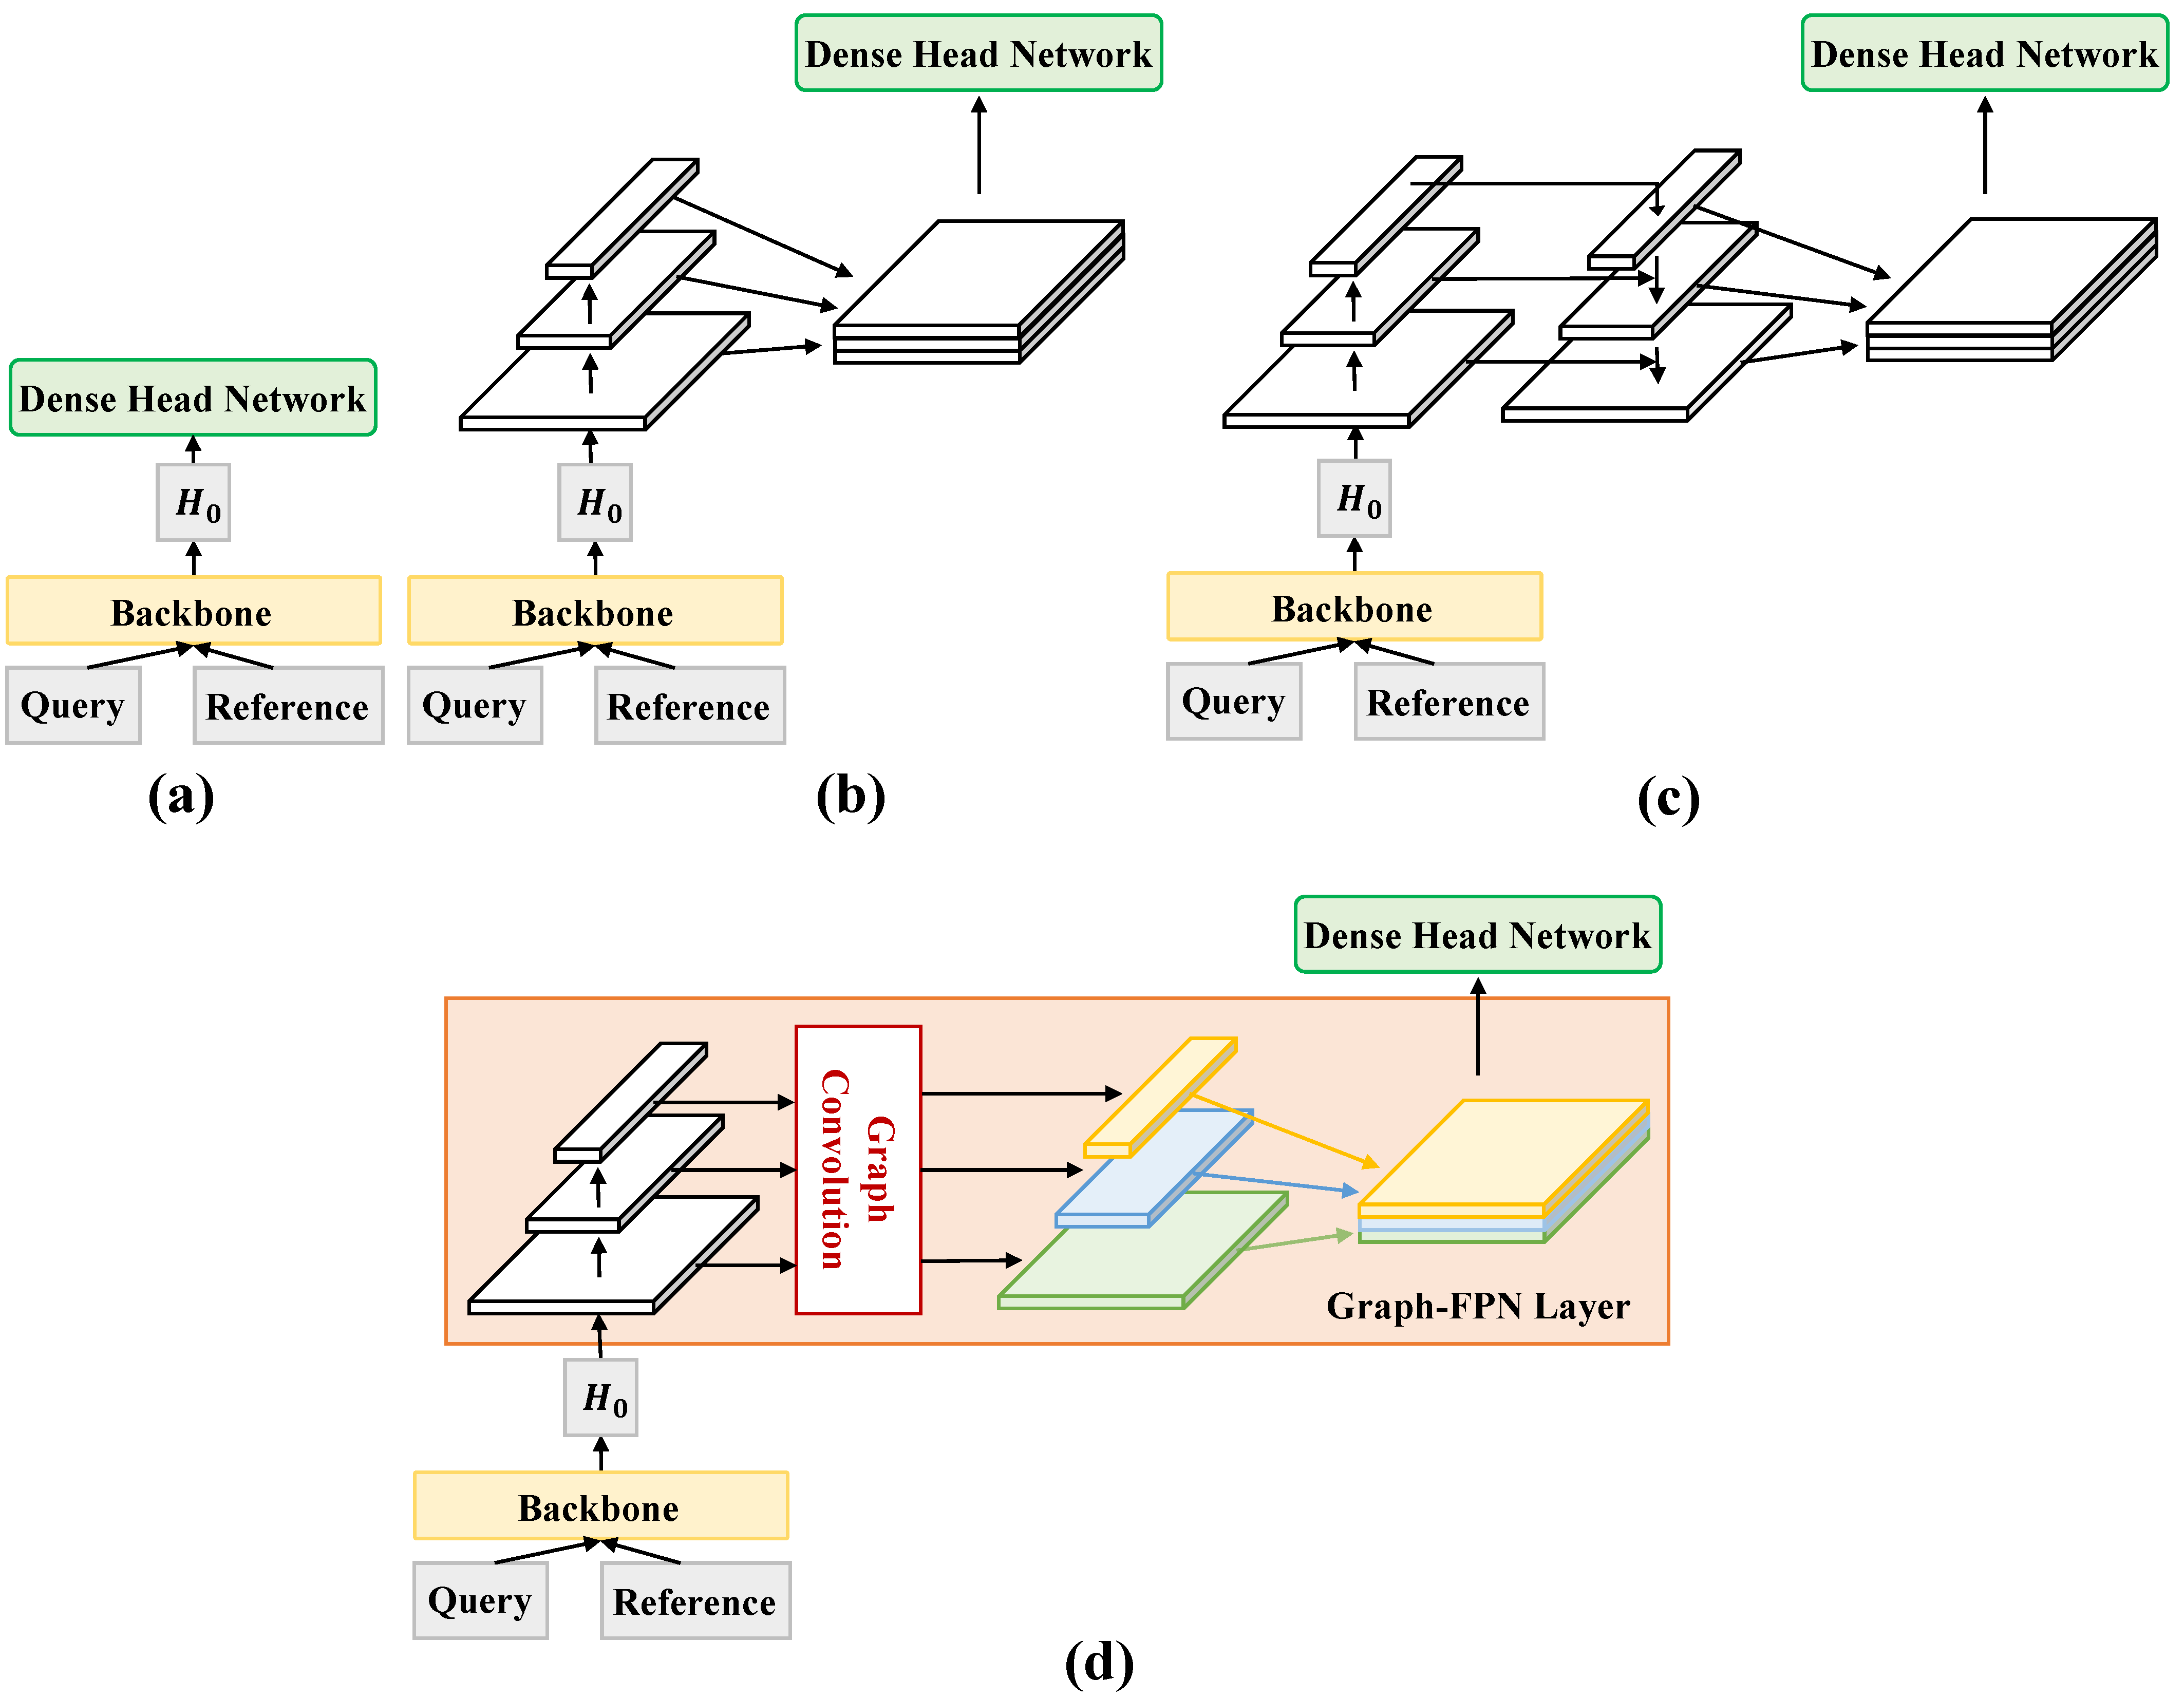
\includegraphics[width=0.9\linewidth]{chapter6/res/ablative_backbone.pdf}
    \caption{同一骨干网络不同特征优化层的性能对比}
    \label{ch6:fig:ablative_backbone}
\end{figure}


\subsection{视频片段检索性能分析}

\textbf{\kaishu{图特征金字塔层的有效性}}:为了验证图特征金字塔层的有效性,我们设计了三种不同的基准模型进行对比。如图~\ref{ch6:fig:ablative_backbone}所示,模型A(a)包含一个骨干网络和一个密集头网络;模型B(b)用骨干网络的输出特征序列构建一个特征金字塔,然后直接将不同尺度的特征直接进行拼接融合;模型C(c)参考FPN(Feature Pyramid Network)~\cite{lin2017feature}使用一个自顶向下的支路网络将不同尺度的特征进行融合;模型D(d)为模型GDP。其中,四个对比模型中的骨干网络和密集头网络结构都完全相同。

%%%%%%%%%% Ablation about Backbone NLVL %%%%%%%%%%%%%%%%
\begin{table*}[t]
    \centering
    \scalebox{0.9}{
        \begin{tabular}{|c | c c c c| c c c c| c c c c|}
            \hline
            & \multicolumn{4}{c|}{TACoS} & \multicolumn{4}{c|}{Charades-STA} & \multicolumn{4}{c|}{ActivityNet Captions}  \\
            \hline
            \multirow{2}{*}{Model} & \multicolumn{3}{c|}{IoU@} & \multirow{2}{*}{mIoU} & \multicolumn{3}{c|}{IoU@} & \multirow{2}{*}{mIoU} & \multicolumn{3}{c|}{IoU@} & \multirow{2}{*}{mIoU} \\
            & 0.1 & 0.3 & 0.5 & \multicolumn{1}{|c|}{} & 0.3 & 0.5 & 0.7 & \multicolumn{1}{|c|}{}  & 01. & 0.3 & 0.5 & \multicolumn{1}{|c|}{} \\
            \hline
            A & 37.4 & 23.3 & 11.5 & 15.3 & 51.8 & 38.3 & 17.8 & 35.1 & 72.1 & 56.0 & \textbf{40.7} & 39.3  \\
            B & 37.3 & 23.1 & \textbf{13.9} & 15.8 & 53.8 & 38.6 & 18.4 & 36.0 & 73.1 & 56.2 & 40.3 & 39.5  \\
            C & 36.8 & 23.1 & 13.8 & 15.7  & 52.6 & 38.9 & 18.3 & 35.8 & 73.7 & 54.7 & 38.9 & 39.4 \\
            D & \textbf{39.7} & \textbf{24.1} & 13.5 & \textbf{16.2} & \textbf{54.5} & \textbf{39.5} & \textbf{18.5} & \textbf{36.6} & \textbf{75.0} & \textbf{56.2} & 39.3 & \textbf{39.8} \\
            \hline
        \end{tabular}
    }       
    \caption{基于语句查询的视频片段检索任务中模型A、B、C、D的性能对比}
    \label{ch6:tab:nlvl_ablation_backbone}
\end{table*}

%%%%%%%%%% Ablation about Backbone VRL %%%%%%%%%%%%%%%
\begin{table*}[t]
    \centering
    \scalebox{0.9}{
        \begin{tabular}{|c |c c c c c|}
            \hline
            mAP@1 & 0.5 & 0.6 & 0.7 & 0.8 & 0.9 \\
            \hline
            A & 41.1 & 34.2 & 27.7  & \textbf{20.3} & 6.8 \\
            B & 43.3 & 35.0 & \textbf{27.9} & 18.2  & 9.6 \\
            C & 42.9 & 34.5 & 26.9 & 18.8  & 8.4 \\
            D & \textbf{44.0} & \textbf{35.4} & 27.7 & 20.0 & \textbf{12.1} \\
            \hline
        \end{tabular}
    }       
    \caption{基于视频查询的视频片段检索任务中模型A、B、C、D的性能对比}
    \label{ch6:tab:vrl_ablation_backbone}
\end{table*}

\begin{figure}[t]
    \centering
    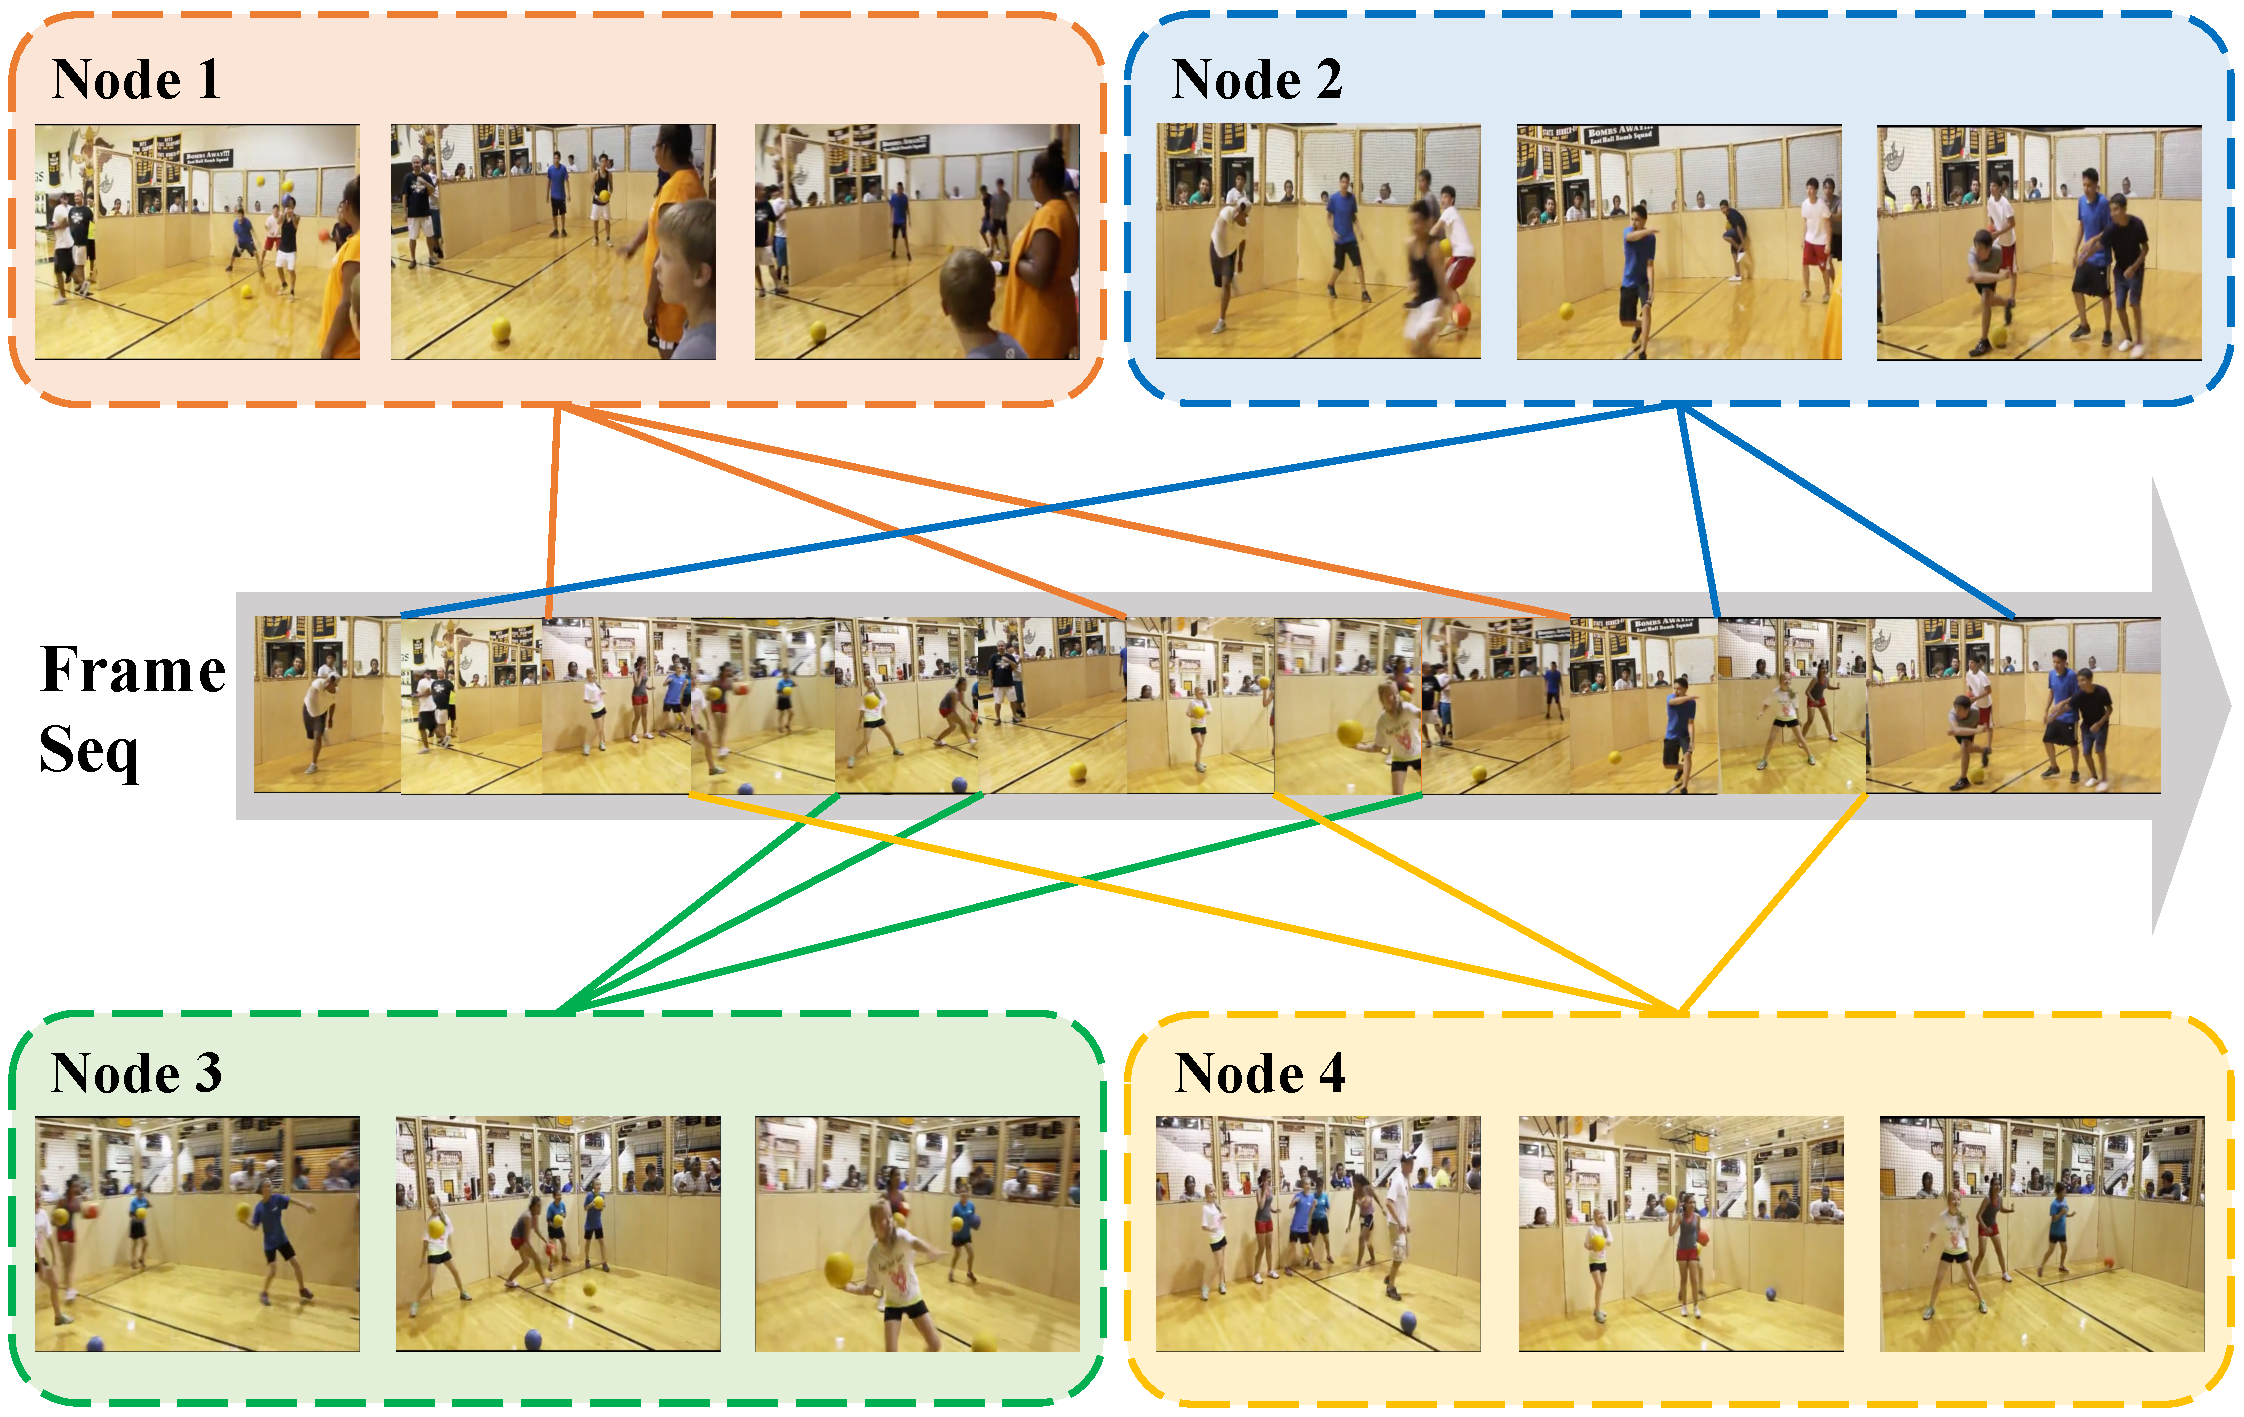
\includegraphics[width=0.9\linewidth]{chapter6/res/node_visualization.pdf}
    \caption{场景空间中的节点可视化示例}
    \label{ch6:fig:node_visualization}
\end{figure}

基于语句查询和视频查询的视频片段检索的结果分别展示在表~\ref{ch6:tab:nlvl_ablation_backbone}和表~\ref{ch6:tab:vrl_ablation_backbone}中。根据实验结果,我们可以发现:(1)特征金字塔结构可以显著地提升视频片段检索任务的性能(即:模型B、C、D的性能明显好于模型A的性能)。(2)利用自顶向下的支路将连续两个尺度的特征进行融合并不能有效地融合多尺度特征。例如,模型B和模型C的性能十分接近,即自顶向下支路和直接拼接效果十分接近。(3)模型GDP(模型D)在绝大多数的数据集和评价指标下都能取得最好的结果,说明了图特征金字塔层对视频检索任务的有效性。


%%%%%%%%%%%%%%%% Ablation Head Network %%%%%%%%%%%%%%
\begin{table}[t]
    \centering
    \scalebox{0.9}{
        \begin{tabular}{|l|l| c c c|}
            \hline
            Dataset & Metric & Sparse & Dense$^*$ & Dense \\
            \hline
            \multirow{4}{*}{TACoS} & IoU@0.1 & 32.3 & 36.5 & \textbf{39.7} \\
            & IoU@0.3 & 18.7 & 22.9 & \textbf{24.1}  \\
            & IoU@0.5 & 9.6 & 13.0 & \textbf{13.5}  \\
            & mIoU & 12.9 & 15.2 & \textbf{16.2}  \\
            \cline{1-5}
            \multirow{4}{*}{Charades-STA} & IoU@0.3 & 52.9 & 53.9 & \textbf{54.5} \\
            & IoU@0.5 & 31.4 & 39.0 & \textbf{39.5}   \\
            & IoU@0.7 & 14.7 & 18.3 & \textbf{18.5} \\
            & mIoU & 35.1 & 36.1 & \textbf{36.6}  \\
            \cline{1-5}
            \multirow{4}{*}{ActivityNet Captions} & IoU@0.1 & 72.4 & 73.5 & \textbf{75.0}  \\
            & IoU@0.3 & 53.0 & 55.9 & \textbf{56.2} \\
            & IoU@0.5 & 37.5 & \textbf{39.8} & 39.3  \\
            & mIoU & 39.0 & 39.3 & \textbf{39.8}  \\
            \hline
            \multirow{6}{*}{ActivityNet-VRL} & tIoU@0.5 & 41.6 & 42.3 & \textbf{44.0}  \\
            & tIoU@0.6 & 30.5 & 35.3 & \textbf{35.4}   \\
            & tIoU@0.7 & 25.7 & 27.6 & \textbf{27.7} \\
            & tIoU@0.8 & 19.8 & \textbf{20.6} & 20.0 \\
            & tIoU@0.9 & 8.5 & \textbf{12.5} & 12.1 \\
            & Average & 25.2 & 27.7 & \textbf{27.8}  \\
            \hline
        \end{tabular}
    }
    \caption{密集型头网络和稀疏型头网络的性能对比}
    \label{ch6:tab:ablation_head}
\end{table}


\textbf{\kaishu{密集头网络的有效性}}:为了评估密集头网络的有效性,我们设计了一个基准对比模型:它使用和模型GDP完全相同的骨干网络和图卷积特征层,然后只是将密集头网络替换成稀疏型头网络,即直接预测两端边界的概率。

基于语句查询和视频查询的视频片段检索的结果展示在表~\ref{ch6:tab:ablation_head}中,其中Sparse表示基准模型(稀疏型头网络),Dense$^*$表示模型在测试阶段没有使用时域池化(图~\ref{ch6:fig:temporal_pooling})。由表~\ref{ch6:tab:ablation_head}可以看出,密集头网络可以显著提升模型性能。尤其对于长视频(如:数据集TACoS),性能提升更加明显。这也间接说明密集头网络能够缓解稀疏头网络中存在的正负训练样本极度不均等问题。


\textbf{\kaishu{场景空间节点的可视化}}:在图~\ref{ch6:fig:node_visualization}中,我们随机选取了同一个尺度下的四个节点进行可视化,其中每个节点选取了三个视频帧来表示节点信息。如图~\ref{ch6:fig:node_visualization}所示,同一个节点中的视频帧通常包含一个特定的视觉场景或相似的场景内容。

\section{本章小结}
在本章,我们深入分析了目前视频片段检索方法的优缺点,并针对稀疏型自底向上框架的设计缺点,提出了一种全新的密集型自底向上网络:基于图特征金字塔的密集型预测(GDP)。模型GDP通过引入一个图特征金字塔层来充分编码视频中多个场景之间的内在联系,提升特征帧序列的表达能力。同时,模型GDP将目前的稀疏头网络替换成密集头网络,不仅可以避免训练过程中正负样本极度不均的问题,同时可以将动作边界预测问题分解成相关性预测和动作边界回归两个子问题,简化视频片段检索的难度。在两种不同的查询形式下(基于自然语句和视频片段)的视频片段检索任务中,模型GDP都能取得当时最好的实验性能。
